\documentclass[10pt, a4paper]{scrartcl}

% --- Pakete ---
\usepackage[utf8]{inputenc}
\usepackage[T1]{fontenc}
\usepackage[ngerman]{babel}
\usepackage{mathptmx}       % Times New Roman
\usepackage{graphicx}       % Für Bilder
\usepackage{geometry}       % Ränder
\usepackage{setspace}       % Zeilenabstand
\usepackage{hyperref}       % Links
\usepackage{amsmath}        % Mathe
\usepackage{float}          % Bildplatzierung
\usepackage{caption}
\usepackage{subcaption}     % Bilder nebeneinander
\usepackage{csquotes}       % Anführungszeichen

% --- Layout ---
\geometry{
    left=2.5cm,
    right=2.5cm,
    top=2.5cm,
    bottom=2cm
}
\onehalfspacing
\setlength{\parindent}{0pt}
\setlength{\parskip}{6pt}

% --- Titeldaten ---
\title{Piepmatz Polizei: Entwicklung eines KI-basierten Systems zum akustischen Monitoring europäischer Vogelarten}
\subtitle{Wettbewerb Jugend forscht 2026}
\author{Finn Degen, Jonathan Ledwon}
\date{\today}

\begin{document}

\maketitle
\begin{center}
    
\includegraphics[width=0.6\textwidth]{bird_project_cover.png} \\
    \vspace{0.5cm} % Optional: Adds a little space between image and text
    \footnotesize{\textit{Cover-Design: David May}}
\end{center}
\thispagestyle{empty}
\newpage

% --- Projektüberblick ---
\section*{Projektüberblick}
Vögel zu zählen ist eine mühsame Angelegenheit. Normalerweise stehen Ornithologen stundenlang im Wald und führen Strichlisten. Das ist nicht nur zeitaufwendig, sondern auch ziemlich ungenau, da man nicht überall gleichzeitig sein kann. Unser Projekt „Piepmatz Polizei“ soll das ändern. Wir haben ein System entwickelt, das Vogelstimmen vollautomatisch aufnimmt und mithilfe von Deep Learning klassifiziert.

Dabei setzen wir nicht auf einfache Frequenzanalysen, sondern nutzen moderne Convolutional Neural Networks (CNNs), die auf Mel-Spektrogrammen trainiert wurden. Wir haben uns dabei nicht auf wenige Garten-Vögel beschränkt, sondern ein Modell trainiert, das einen Großteil der relevanten europäischen Vogelwelt erkennt.
Die Kombination aus etablierten Architekturen wie EfficientNet und experimentellen Ansätzen wie Metric Learning sorgt dafür, dass die KI auch bei Wind oder Verkehrslärm nicht aus dem Tritt kommt. Zusätzlich haben wir ein Gehäuse entworfen, damit die Hardware auch mal einen Regenschauer überlebt.

\newpage
\tableofcontents
\newpage

% --- Inhalt ---

\section{Einleitung: Warum eigentlich Vögel?}
Vögel sind so etwas wie die Sensoren unseres Ökosystems. Wenn es ihnen schlecht geht, stimmt meistens auch etwas mit der Umwelt nicht. Das Problem ist nur die Erfassung. Sie sind scheu, schnell und verstecken sich gerne im Gebüsch. Die akustische Erfassung ist daher der Goldstandard. Menschliche Experten sind aber teuer und können nicht rund um die Uhr im Wald stehen, jedoch sind die Vorteile immens: Migrationsbewegungen oder unbekante Arten erfassen, Bauprojekte die auf das Ökosystem angepasst sind, frühzeitigeres Erkennen von Artensterben, etc.

Unsere Fragestellung war also simpel: Können wir ein Gerät bauen, das wir einfach in den Baum hängen, und das uns am Ende des Monats eine Excel-Tabelle gibt? Wir wollten wissen, wer wann gesungen hat. Uns war schnell klar, dass ein solches System nur dann wirklich nützlich ist, wenn es nicht nur Amsel, Drossel, Fink und Star unterscheidet, sondern die Vielfalt der europäischen Vogelwelt abdeckt. Unser finales Modell ist daher auf über 600 Arten trainiert.

\section{Theoretische Grundlagen}

\subsection{Vom Ton zum Bild: Mel-Spektrogramme}
Computer hören nicht so wie wir Menschen. Wenn wir Audiodaten in ein neuronales Netz füttern wollen, könnten wir zwar die rohe Wellenform verwenden. Das ist aber rechenintensiv und oft ineffizient. Viel besser funktionieren Bilderkennungsnetze (CNNs), die eigentlich für Fotos gemacht sind.
Deshalb wandeln wir den Sound in Bilder um, sogenannte Spektrogramme. Dabei wird die Zeit auf der X-Achse und die Frequenz auf der Y-Achse abgetragen, die Helligkeit des Bildes an dieser Stelle ist dann die Lautstärke/Intensität. 

Wir haben uns intensiv damit beschäftigt, wie man diese Bilder am besten aufbereitet. In Abbildung \ref{fig:mel_vs_lin} sieht man den Vergleich. Oben ist ein lineares Spektrogramm. Unten ist die \textit{Mel-Skala}. Diese Skala ist der menschlichen und vogelartigen Wahrnehmung nachempfunden. Wir hören Unterschiede in tiefen Tönen viel besser als in sehr hohen. Die Mel-Skala „zoomt“ sozusagen in die für Vögel relevanten Bereiche rein. Dadurch sieht das neuronale Netz die feinen Details im Gesang viel besser.

\begin{figure}[H]
    \centering
    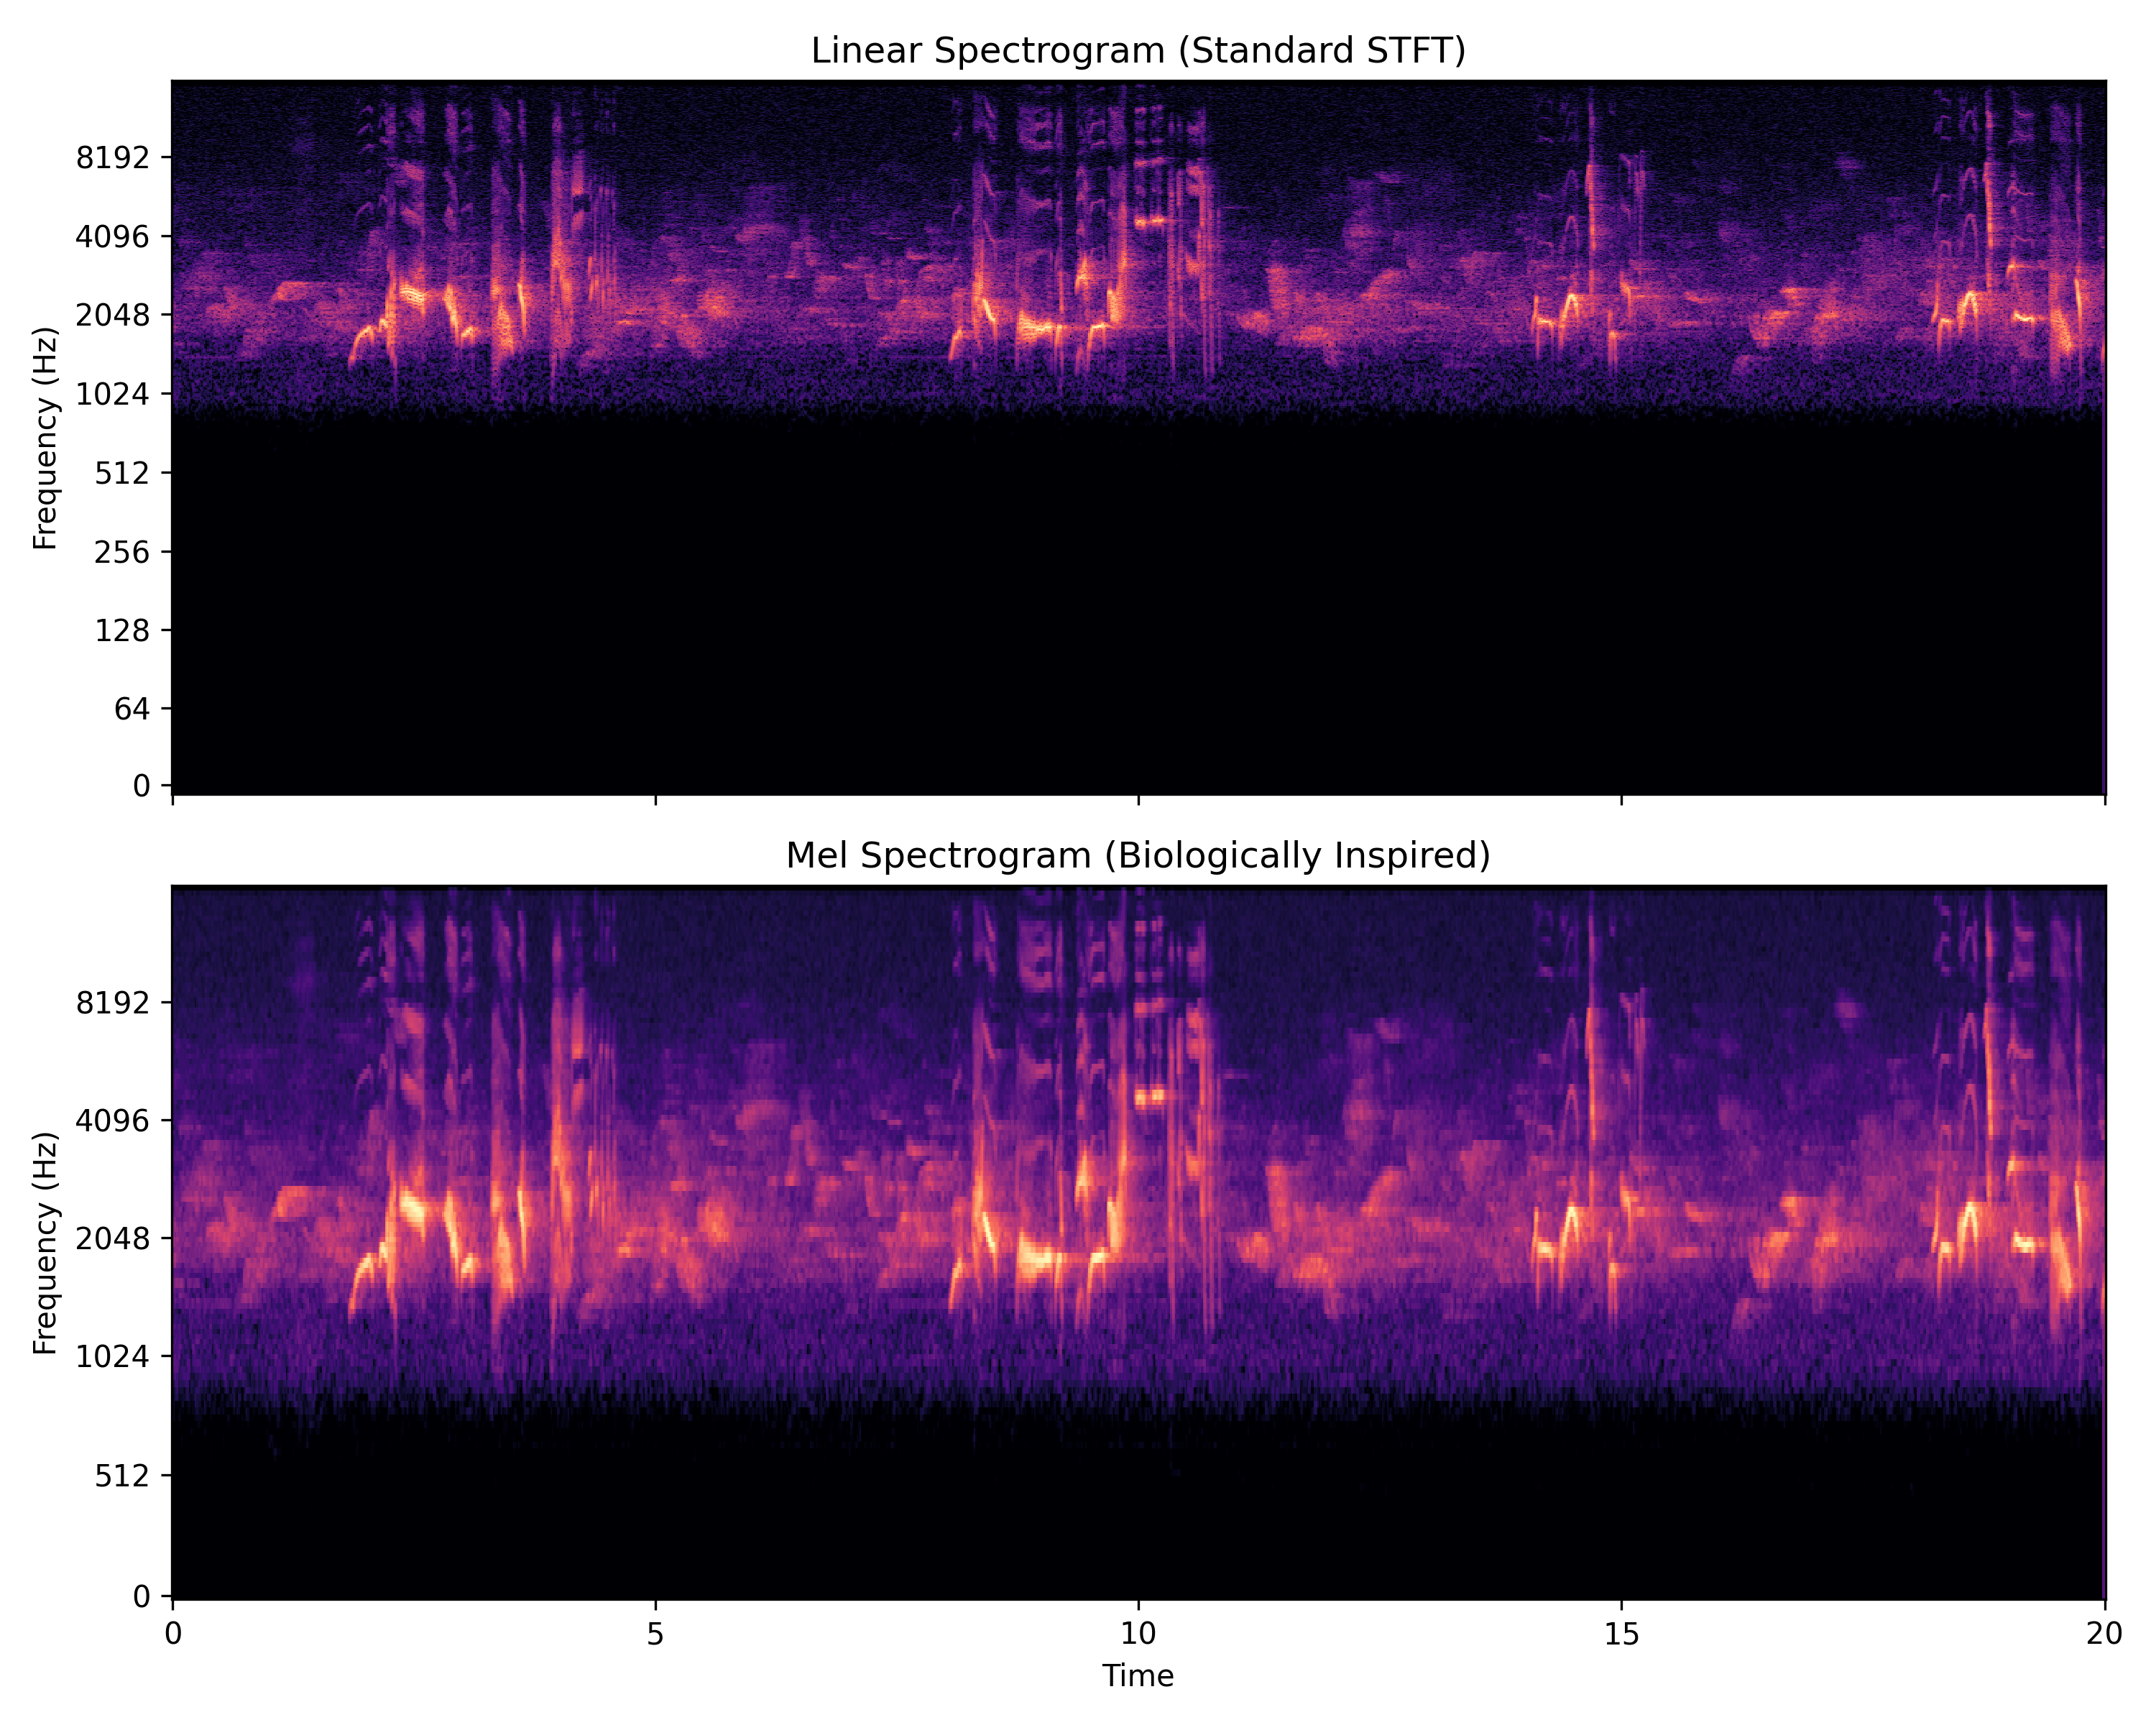
\includegraphics[width=0.85\textwidth]{Pictures/comparison_linear_vs_mel.png}
    \caption{Vergleich der Darstellung: Das Mel-Spektrogramm (unten) löst die für Vögel relevanten Frequenzbereiche deutlich detailierter auf als die lineare Darstellung (oben).}
    \label{fig:mel_vs_lin}
\end{figure}

\subsection{Artenvielfalt im Bild}
Es ist faszinierend zu sehen, wie unterschiedlich die Arten bereits visuell sind. Eine Amsel sieht im Spektrogramm ganz anders aus als ein Haussperling. Abbildung \ref{fig:species_comp} zeigt exemplarisch fünf zufällig ausgewählte Arten aus unserem Datensatz, um die visuelle Unterscheidbarkeit zu demonstrieren.

\begin{figure}[H]
    \centering
    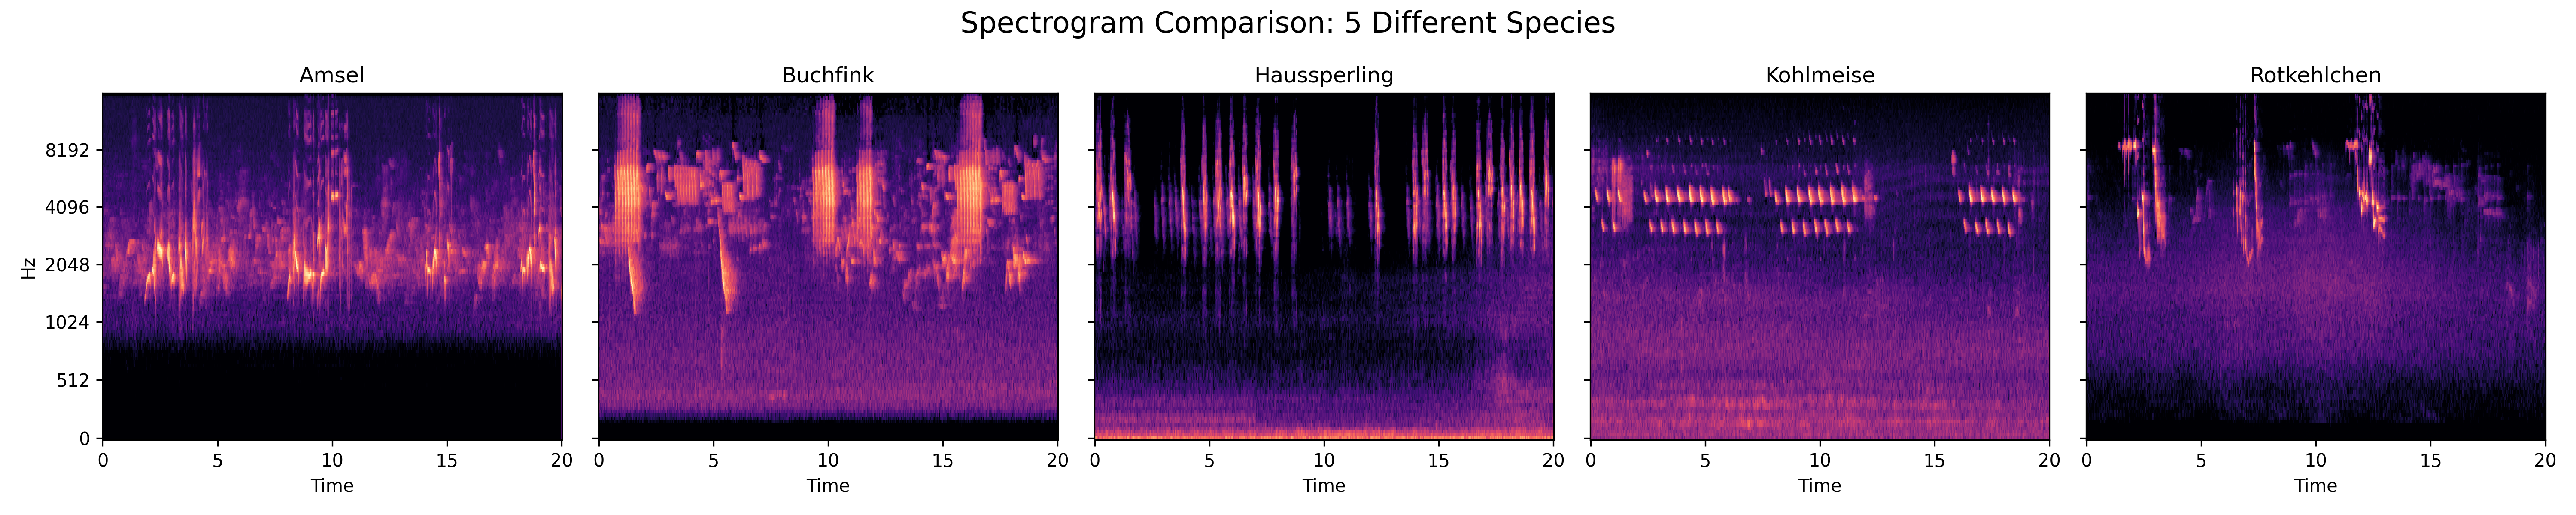
\includegraphics[width=1.0\textwidth]{Pictures/comparison_species.png}
    \caption{Exemplarische Spektrogramme von fünf Arten aus unserem umfangreichen Europa-Datensatz. Die visuellen Strukturen sind deutlich unterscheidbar, was dem CNN die Klassifikation ermöglicht.}
    \label{fig:species_comp}
\end{figure}

\section{Vorgehensweise und Methoden}

\subsection{Datenpipeline: Ein europäischer Datensatz}
Unsere Daten kommen von Xeno-Canto, einer riesigen Datenbank für Vogelstimmen. Um ein wirklich universelles Tool zu schaffen, haben wir unser Download-Skript so programmiert, dass es automatisch Metadaten und Audiofiles für das Verbreitungsgebiet Europa zieht. Das resultiert in einer enormen Menge an Trainingsdaten.

Wichtig war uns dabei unser System so robust wie möglich zu gestalten. Viele Aufnahmen auf Xeno-Canto sind extrem sauber (Richtmikrofone, Qualitätsstufe A). Im echten Wald rauscht es aber. Deshalb haben wir gezielt auch Aufnahmen mit den Qualitätsstufen B und C in den Trainingsdaten gelassen. Das Modell soll ja lernen, Vögel auch bei Hintergrundlärm zu erkennen.

Unsere Pipeline verarbeitet die Daten \textit{on-the-fly}:
\begin{itemize}
    \item Resampling auf 32kHz (mehr brauchen wir für Vögel nicht).
    \item Zerschneiden in 5-Sekunden-Stücke.
    \item Umwandlung in Mel-Spektrogramme (128 Bänder).
    \item Logarithmierung (dB) und Normalisierung auf Werte zwischen 0 und 1.
\end{itemize}

\subsection{Die neuronalen Netzarchitekturen}
Um die Komplexität der europäischen Vogelwelt abzubilden, haben wir nicht nur ein Standard-Modell trainiert, sondern zwei spezialisierte Architekturen entwickelt und evaluiert.

\subsubsection{Der Klassifikator (EfficientNet-B0)}
Für die direkte Bestimmung der Arten nutzen wir ein \textit{EfficientNet-B0}. Diese Architektur wurde von Google entwickelt, um ein optimales Verhältnis zwischen Genauigkeit und Rechenleistung zu bieten – ideal für den späteren Einsatz auf Edge-Geräten wie dem Raspberry Pi.
\begin{itemize}
    \item \textbf{Transfer Learning:} Wir initialisieren das Netz nicht mit zufälligen Werten, sondern nutzen Gewichte, die bereits auf dem riesigen ImageNet-Datensatz (Millionen von Fotos) trainiert wurden. Das Netz „weiß“ also schon, wie man Kanten, Kurven und Texturen sieht. Wir bringen ihm dann nur noch bei, diese visuellen Merkmale als Vogelstimmen zu interpretieren.
    \item \textbf{Output Layer:} Der letzte Layer des Netzes wurde angepasst, um die Wahrscheinlichkeiten für alle trainierten europäischen Arten auszugeben (Softmax-Aktivierung).
\end{itemize}

\subsubsection{Der Embedding-Extraktor (Metric Learning)}
Zusätzlich haben wir mit einem experimentellen Ansatz gearbeitet: \textbf{Metric Learning}. Hierbei klassifiziert das Netz nicht direkt („Das ist eine Amsel“), sondern lernt, ähnliche Gesänge nahe beieinander in einem hochdimensionalen Raum zu platzieren.
\begin{itemize}
    \item \textbf{Projektions-Head:} Statt einer Klassifikationsebene nutzen wir einen Projektions-Head (Linear $\rightarrow$ BatchNorm $\rightarrow$ PReLU $\rightarrow$ Linear), der das Spektrogramm auf einen 512-dimensionalen Vektor abbildet.
    \item \textbf{ArcFace Loss:} Wir trainieren mit der \textit{Sub-Center ArcFace Loss}-Funktion. Diese zwingt das Netz, die Vektoren auf einer Hypersphäre so anzuordnen, dass Gesänge derselben Art extrem nah beieinander liegen (kleiner Winkelabstand) und verschiedene Arten maximalen Abstand haben.
    \item \textbf{Vorteil:} Dieser Ansatz erlaubt es uns, eine „Landkarte der Biodiversität“ zu erstellen und potenziell sogar Arten zu erkennen, die gar nicht im Training dabei waren (Out-of-Distribution Detection), indem man prüft, ob ein neuer Vektor in keinen bekannten Cluster passt.
\end{itemize}

\subsection{Trainingstrategie}
Um das Modell bei dieser enormen Anzahl an Klassen robust zu machen, haben wir tief in die Trickkiste der Regularisierung gegriffen. Besonders wichtig war uns \textbf{SpecAugment}. Dabei löschen wir im Training einfach zufällig Teile des Spektrogramms. Mal fehlen ein paar Millisekunden, mal fehlt ein Frequenzbereich. Das zwingt das Netz, den Vogel auch dann zu erkennen, wenn er nur teilweise zu hören ist und macht das Modell somit weniger anfällig auf Störgeräusche.

Wir haben den Trainingsverlauf genau überwacht. In Abbildung \ref{fig:loss_curve} sieht man, wie der Fehler (Loss) über die Epochen abnimmt. Man erkennt gut, dass das Modell stetig lernt, ohne dabei zu starke Ausreißer zu haben.

\begin{figure}[H]
    \centering
    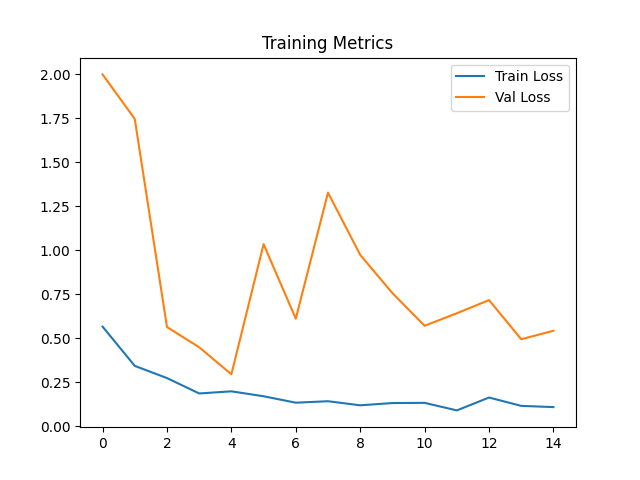
\includegraphics[width=0.7\textwidth]{Pictures/loss_curve_15epoch_resnet18pre.png}
    \caption{Erste 15 Eopchen vom Trainingsverlauf: Normalerweise ist es ein Anzeichen von Overfitting wenn Val Loss deutlich höher als Train Loss ist, aber bei uns ist der Grund hierfür, dass wir Noise hinzufügen und diese hier sichtbar wird.}
    \label{fig:loss_curve}
\end{figure}

\section{Ergebnisse: Wie gut funktioniert es?}

\subsection{Trefferquote und Vergleich}
Ehrlich gesagt waren wir selbst überrascht. Unser finales Modell (EfficientNet mit Transfer Learning) erreicht extrem hohe Genauigkeiten, und das obwohl es hunderte verschiedene Arten unterscheiden muss.
Zum Vergleich haben wir ein Modell komplett von Null trainiert („From Scratch“). Das kam nur auf ca. 80\% und hat extrem schnell angefangen, die Trainingsdaten auswendig zu lernen. Transfer Learning ist hier also der absolute Gamechanger, wie man in Abbildung \ref{fig:modelcomp} sieht. Die Tatsache, dass wir das Modell so stark skalieren konnten, ohne massiv an Genauigkeit zu verlieren, bestätigt unseren Ansatz.

\begin{figure}[H]
    \centering
    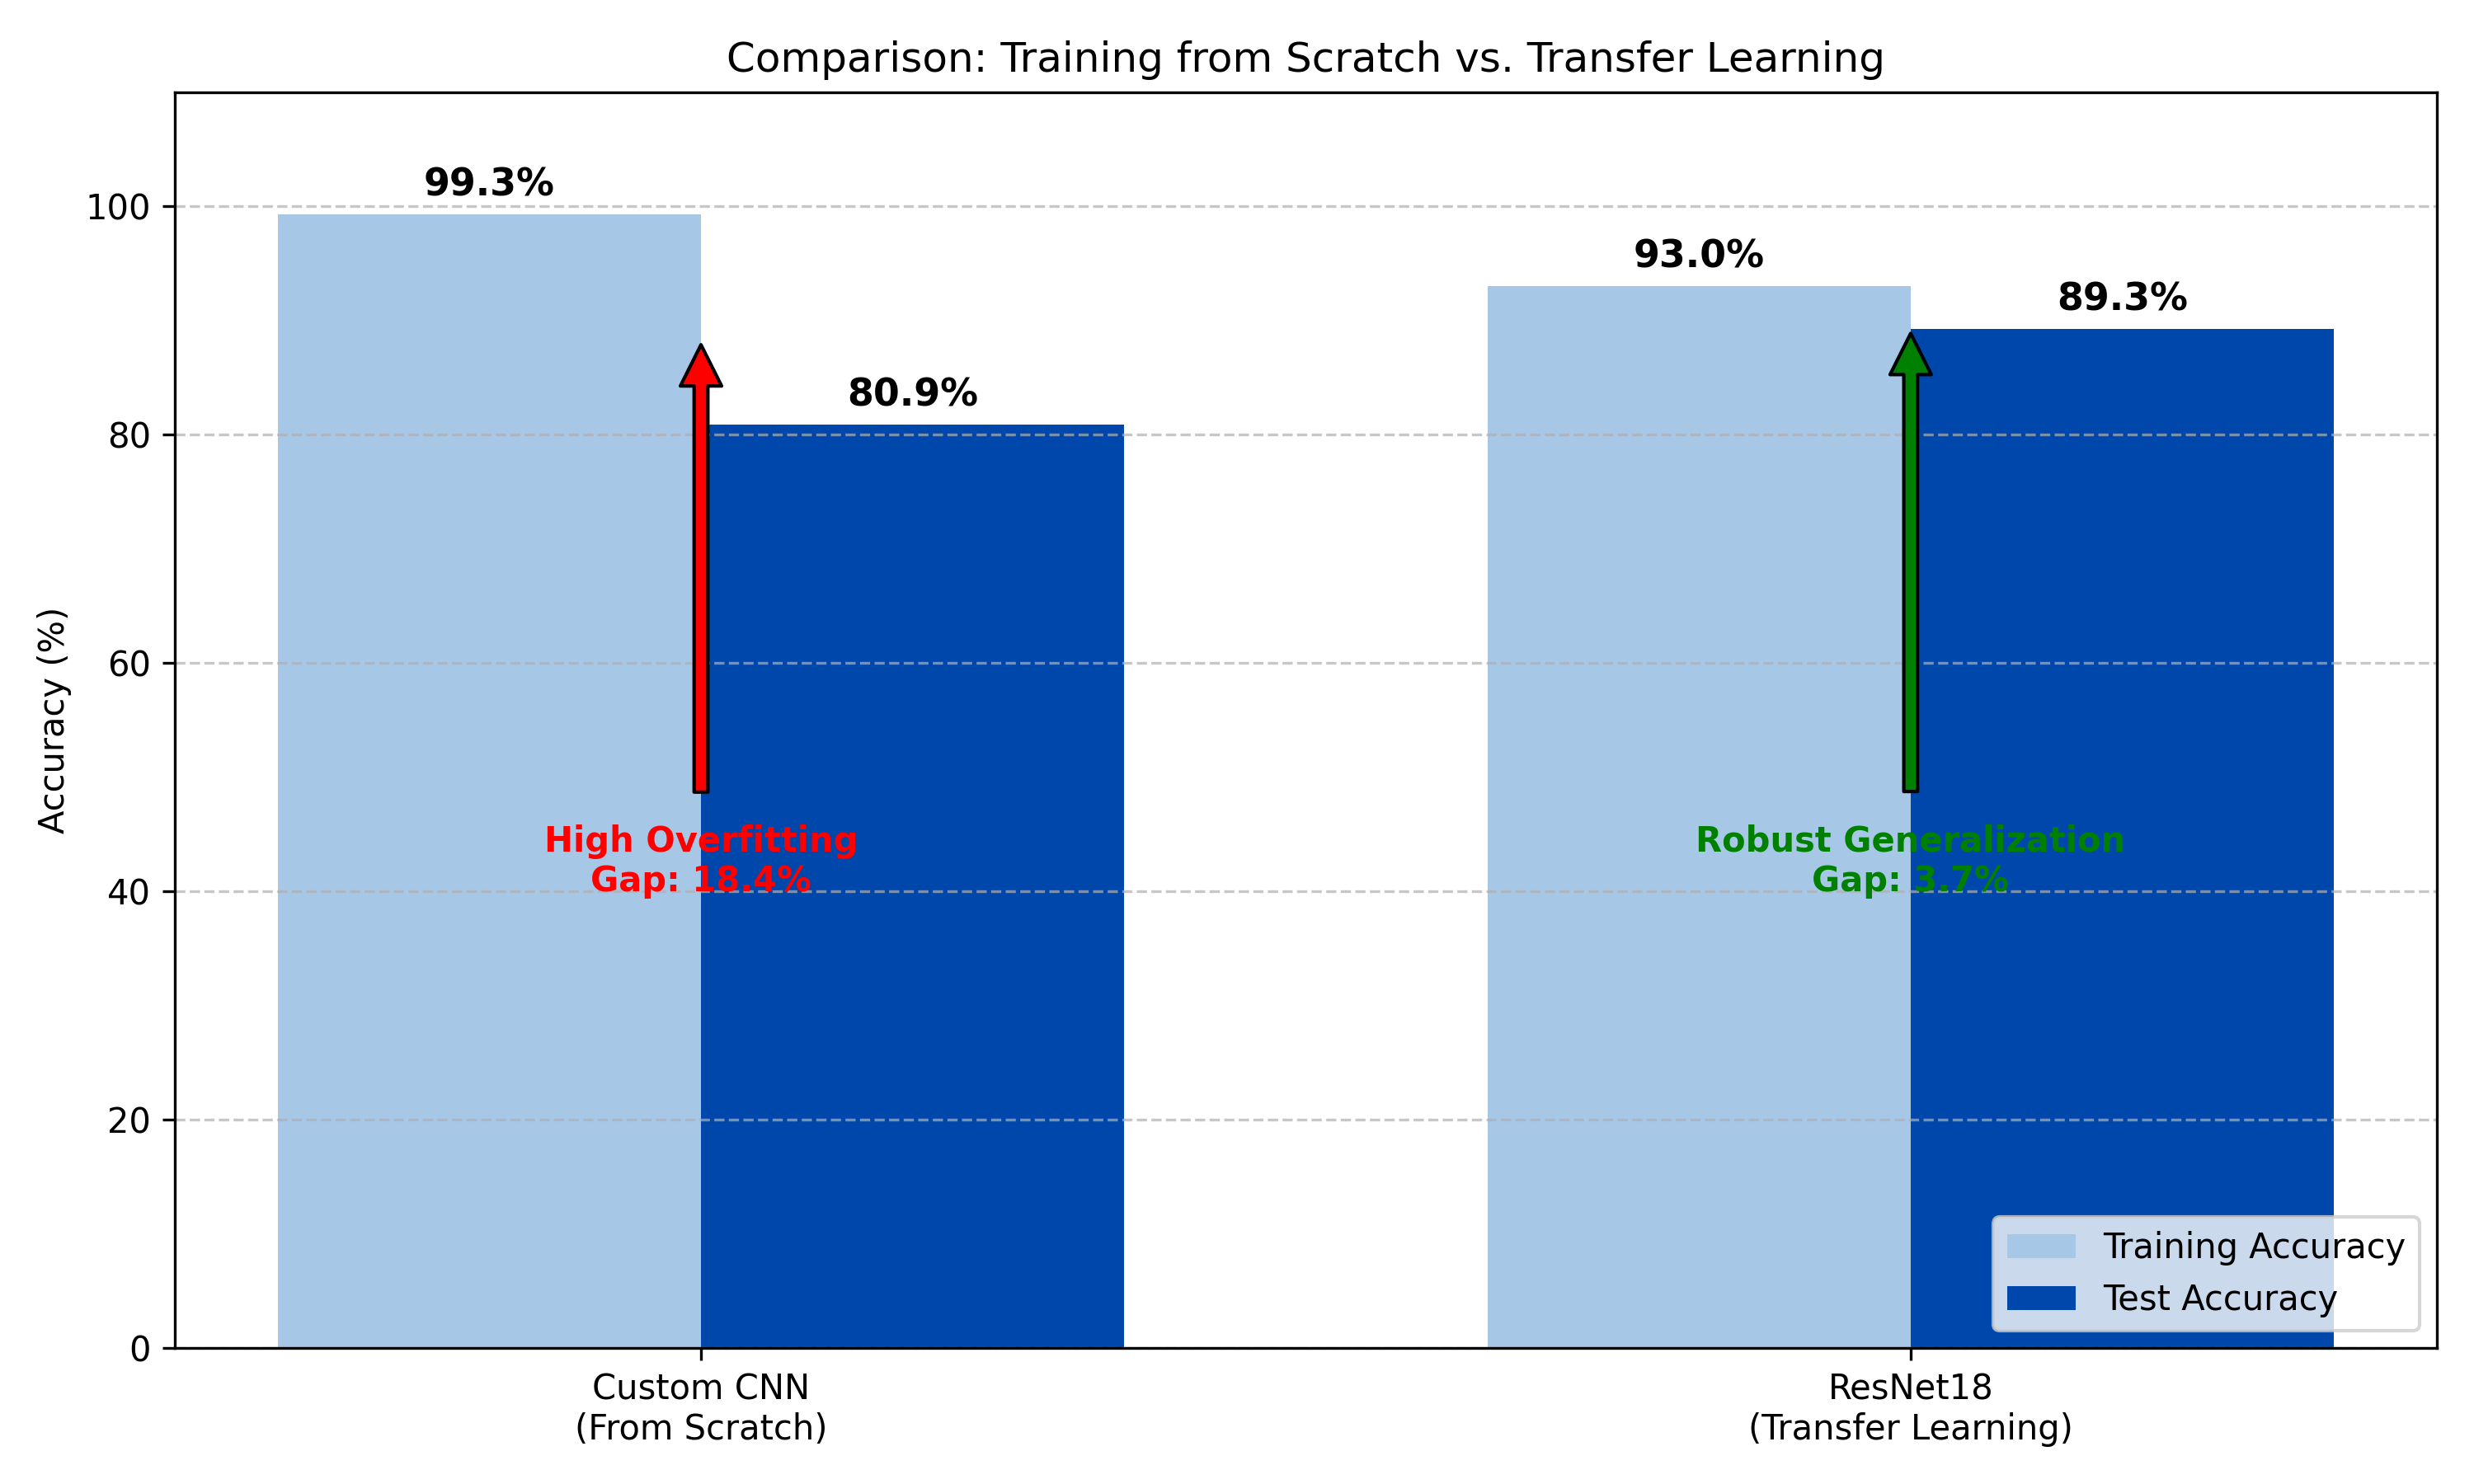
\includegraphics[width=0.7\textwidth]{Pictures/comparison_model_performance.png}
    \caption{Der Vergleich zeigt deutlich: Das Transfer-Learning-Modell (rechts) ist nicht nur präziser, sondern generalisiert auch besser auf neue Daten, selbst bei vielen Klassen.}
    \label{fig:modelcomp}
\end{figure}

Ein wichtiger Faktor für die Genauigkeit ist die verfügbare Datenmenge pro Vogelart. Abbildung \ref{fig:bubble} zeigt, dass unsere Methode ihr Ziel erreicht hat, öfter mit den Daten seltener Vögel zu trainieren und die KI nun auch seltene Vogelarten gut erkennt.

\begin{figure}[H]
    \centering
    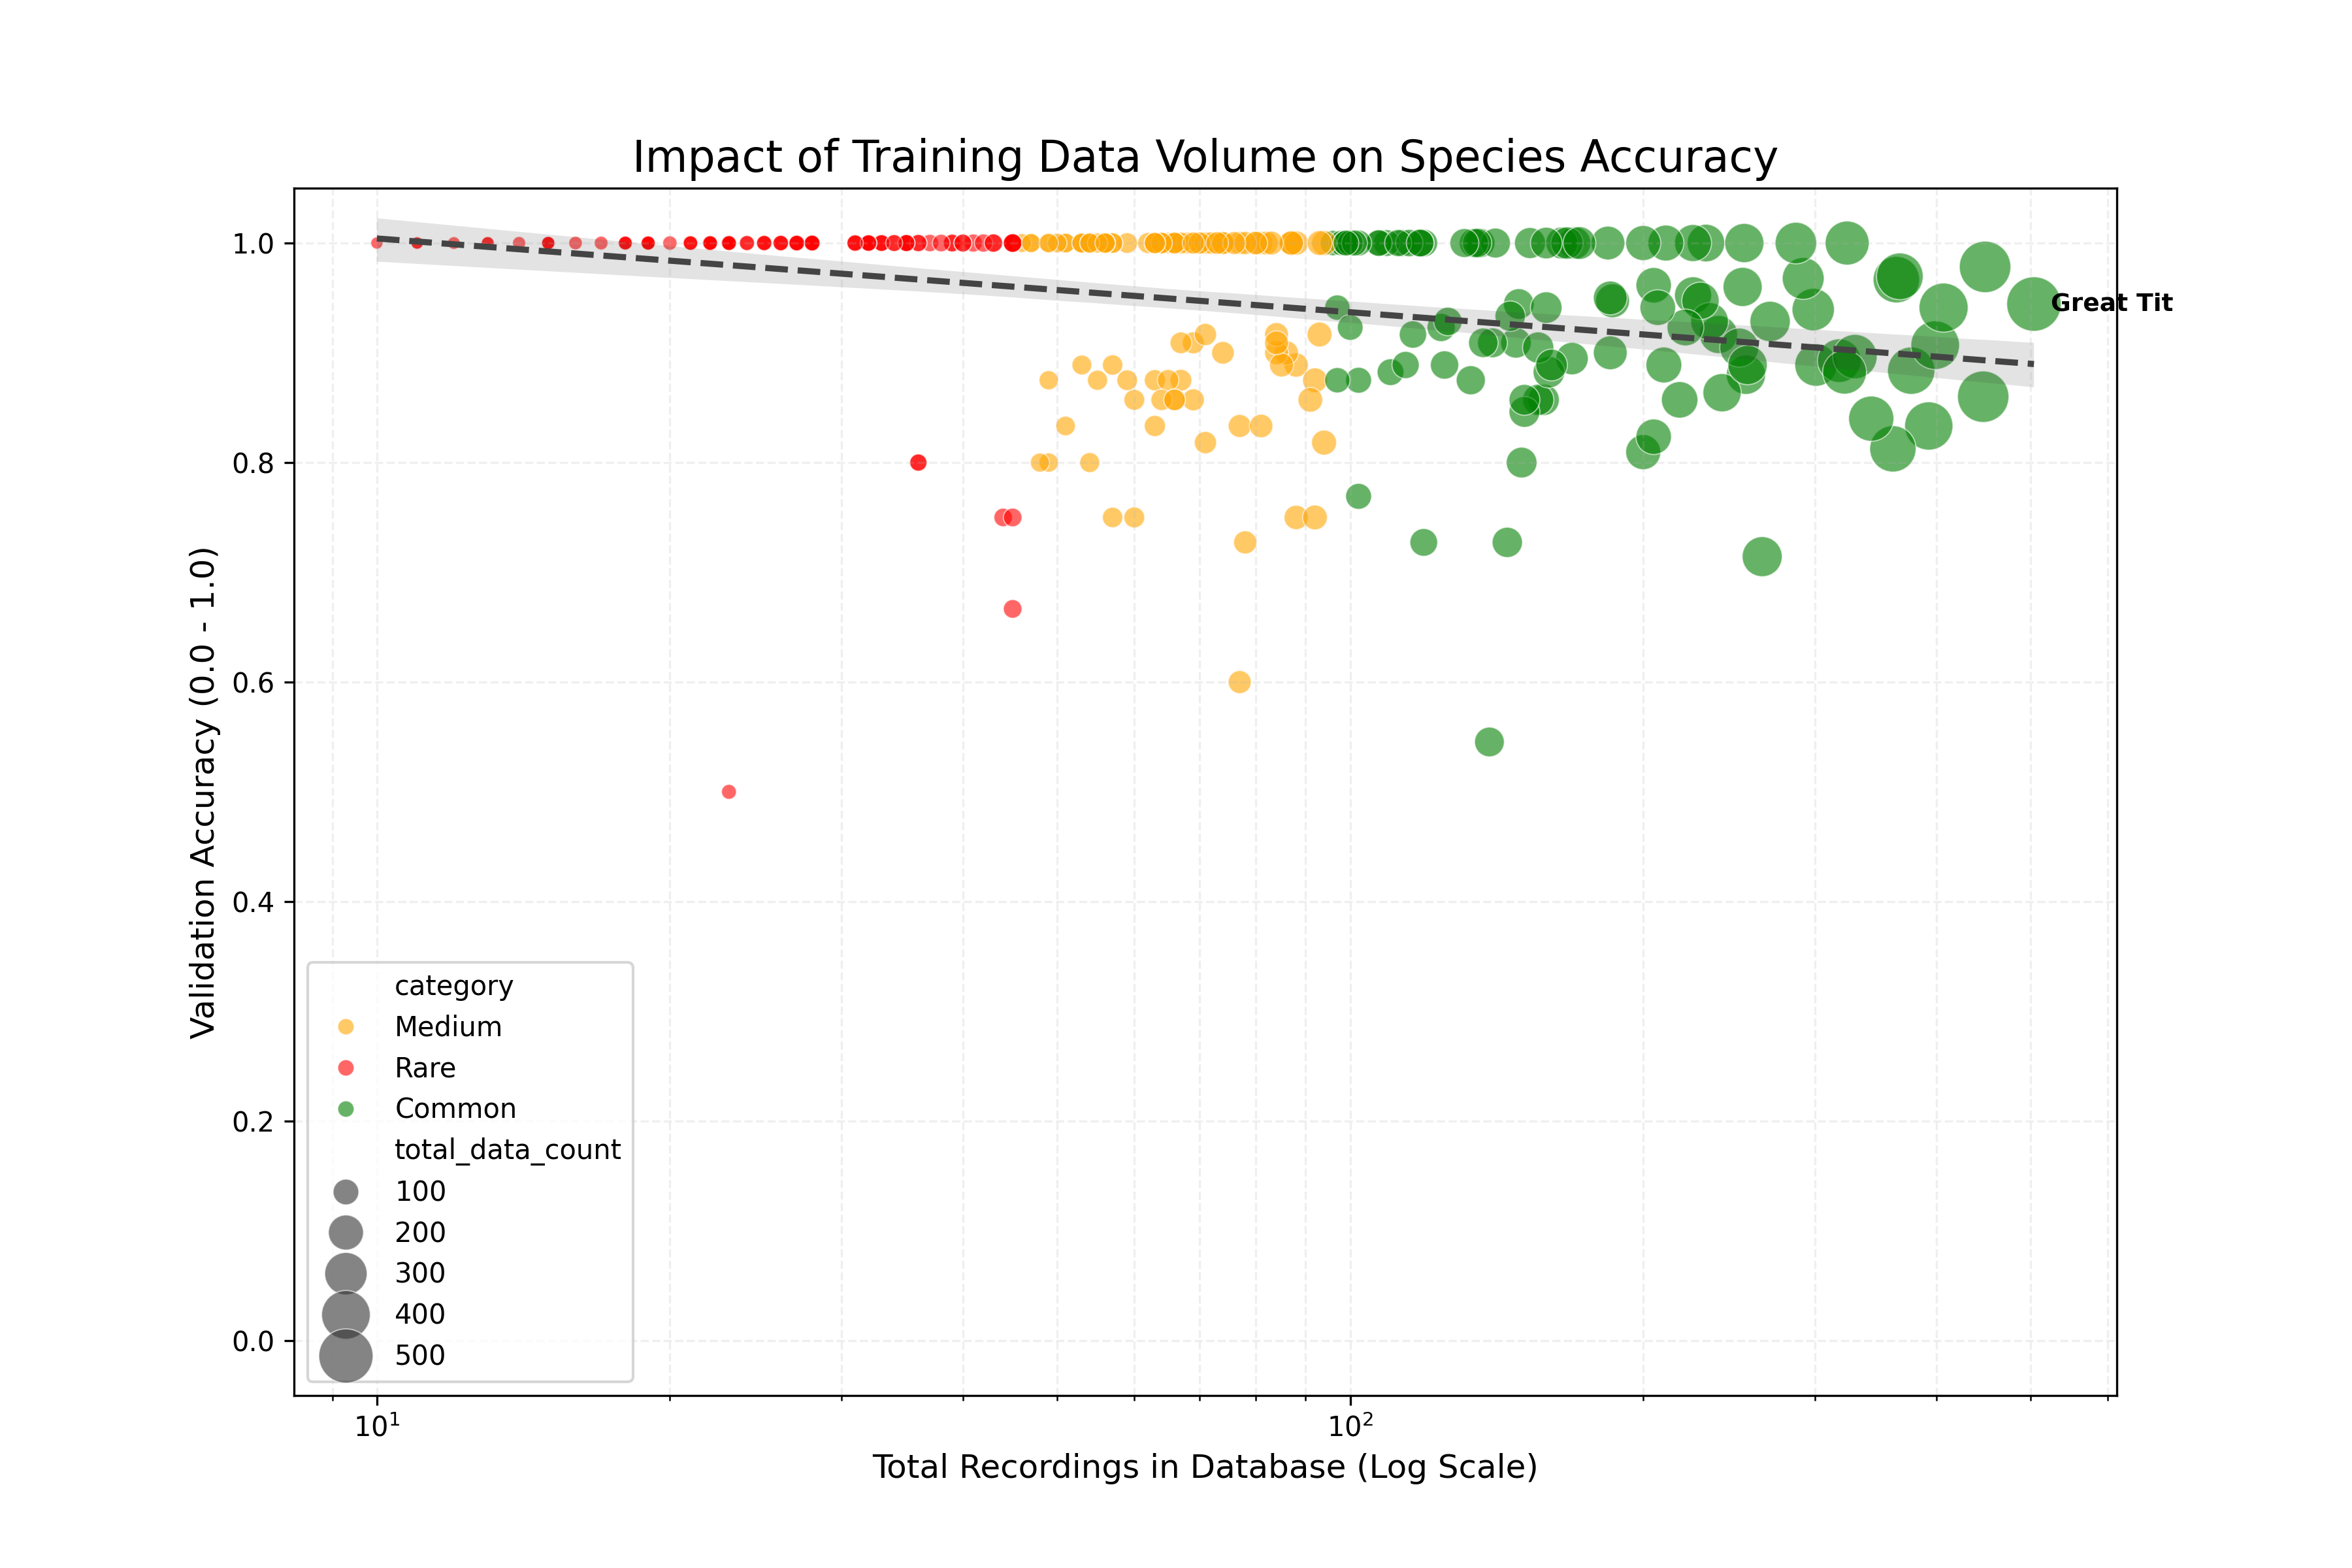
\includegraphics[width=0.8\textwidth]{Pictures/scatter_data_vs_acc_bubble.png}
    \caption{Einfluss der Datenmenge auf die Genauigkeit. Die Größe der Blasen repräsentiert die Anzahl der Trainingsdaten.}
    \label{fig:bubble}
\end{figure}


\subsection{Fehleranalyse}
Natürlich ist keine KI perfekt. Wir haben die Fehler genau analysiert. Die Konfusionsmatrix in Abbildung \ref{fig:conf_matrix} zeigt exemplarisch einen Ausschnitt der Ergebnisse. Die Diagonale ist dunkelgrün, was exemplarisch für eine hohe Genauigkeit ist. Verwechslungen treten vor allem bei sehr kurzen Rufen von verwandten Arten auf (z.B. verschiedene Finken-Arten). Das ist aber auch für menschliche Experten oft schwer zu unterscheiden, außerdem war die richtige Art mit über 99\%iger Wahrscheinlichkeit in den Top-3.

\begin{figure}[H]
    \centering
    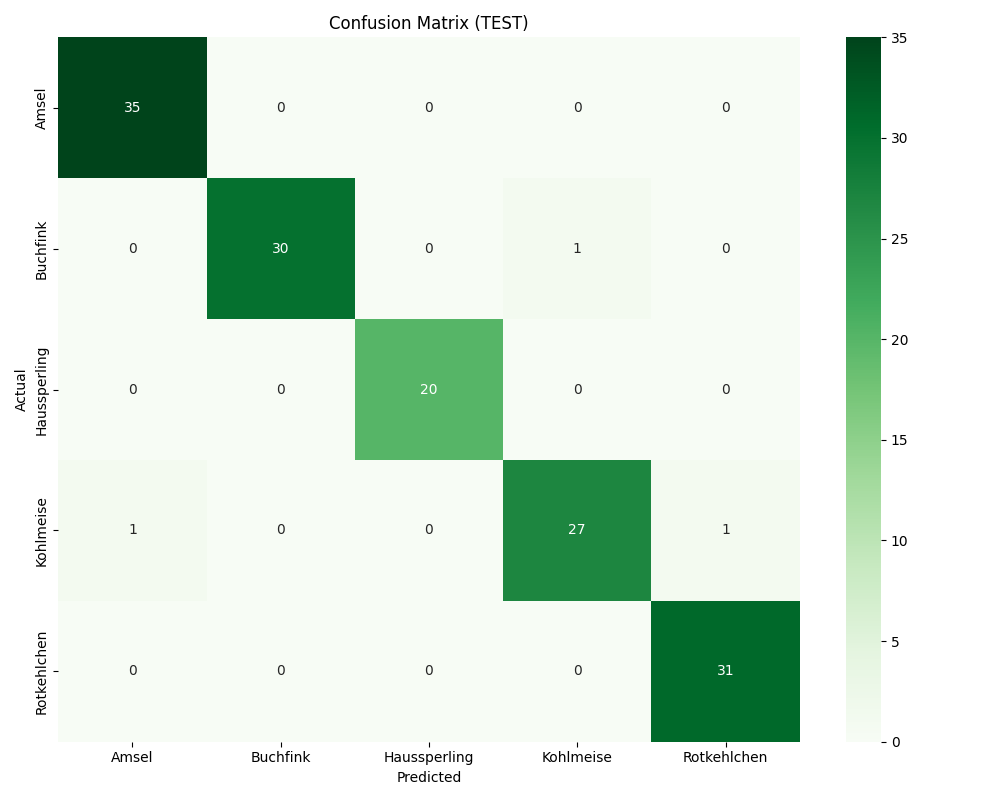
\includegraphics[width=0.6\textwidth]{Pictures/confusion_matrix_finetuned_pro.png}
    \caption{Konfusionsmatrix des finalen Modells (Ausschnitt). Die hohen Zahlen auf der Diagonale bestätigt die hohe Präzision auch bei vielen unterschiedlichen Klassen.}
    \label{fig:conf_matrix}
\end{figure}

In Abbildung \ref{fig:top_errors} haben wir die häufigsten Fehlklassifikationen genauer aufgeschlüsselt.

\begin{figure}[H]
    \centering
    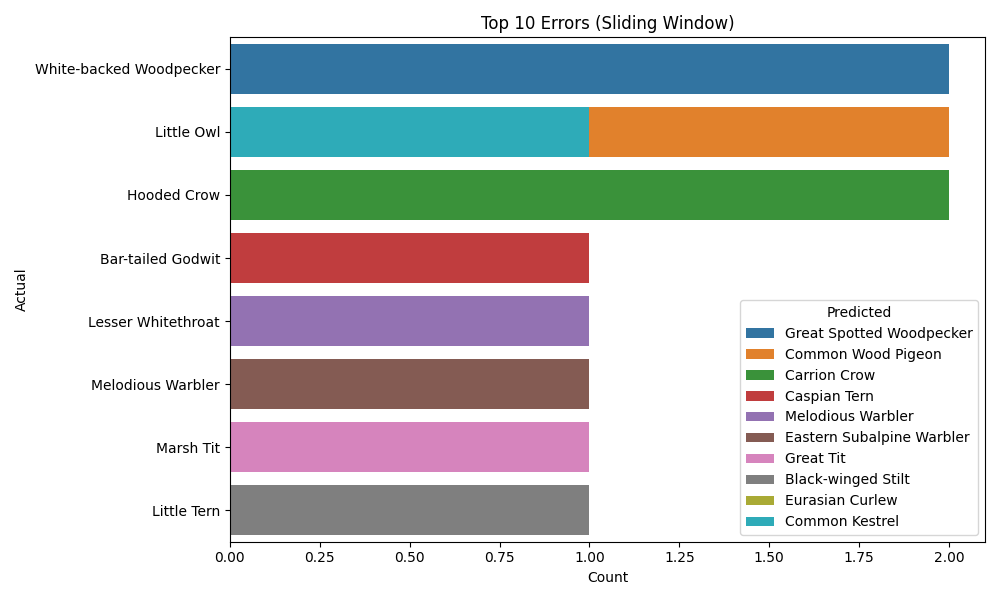
\includegraphics[width=0.8\textwidth]{Pictures/top_errors.png}
    \caption{Die häufigsten Verwechslungen. Balken zeigen an, welche Art fälschlicherweise als welche andere Art klassifiziert wurde.}
    \label{fig:top_errors}
\end{figure}

%TODO: change image
\subsection{Robustheit gegen schlechte Audioqualität}
Ein wichtiger Punkt war uns die Frage, wie das Modell reagiert, wenn die Aufnahmequalität sinkt. Auf Xeno-Canto sind die Aufnahmen mit Buchstaben von A (Studio) bis E (unbrauchbar) bewertet.
In Abbildung \ref{fig:quality} sehen wir, dass die Erkennungsrate bei A-C ungefähr gleichbleibt, unser Modell ist also relativ unabhängig von Audioqualität.

\begin{figure}[H]
    \centering
    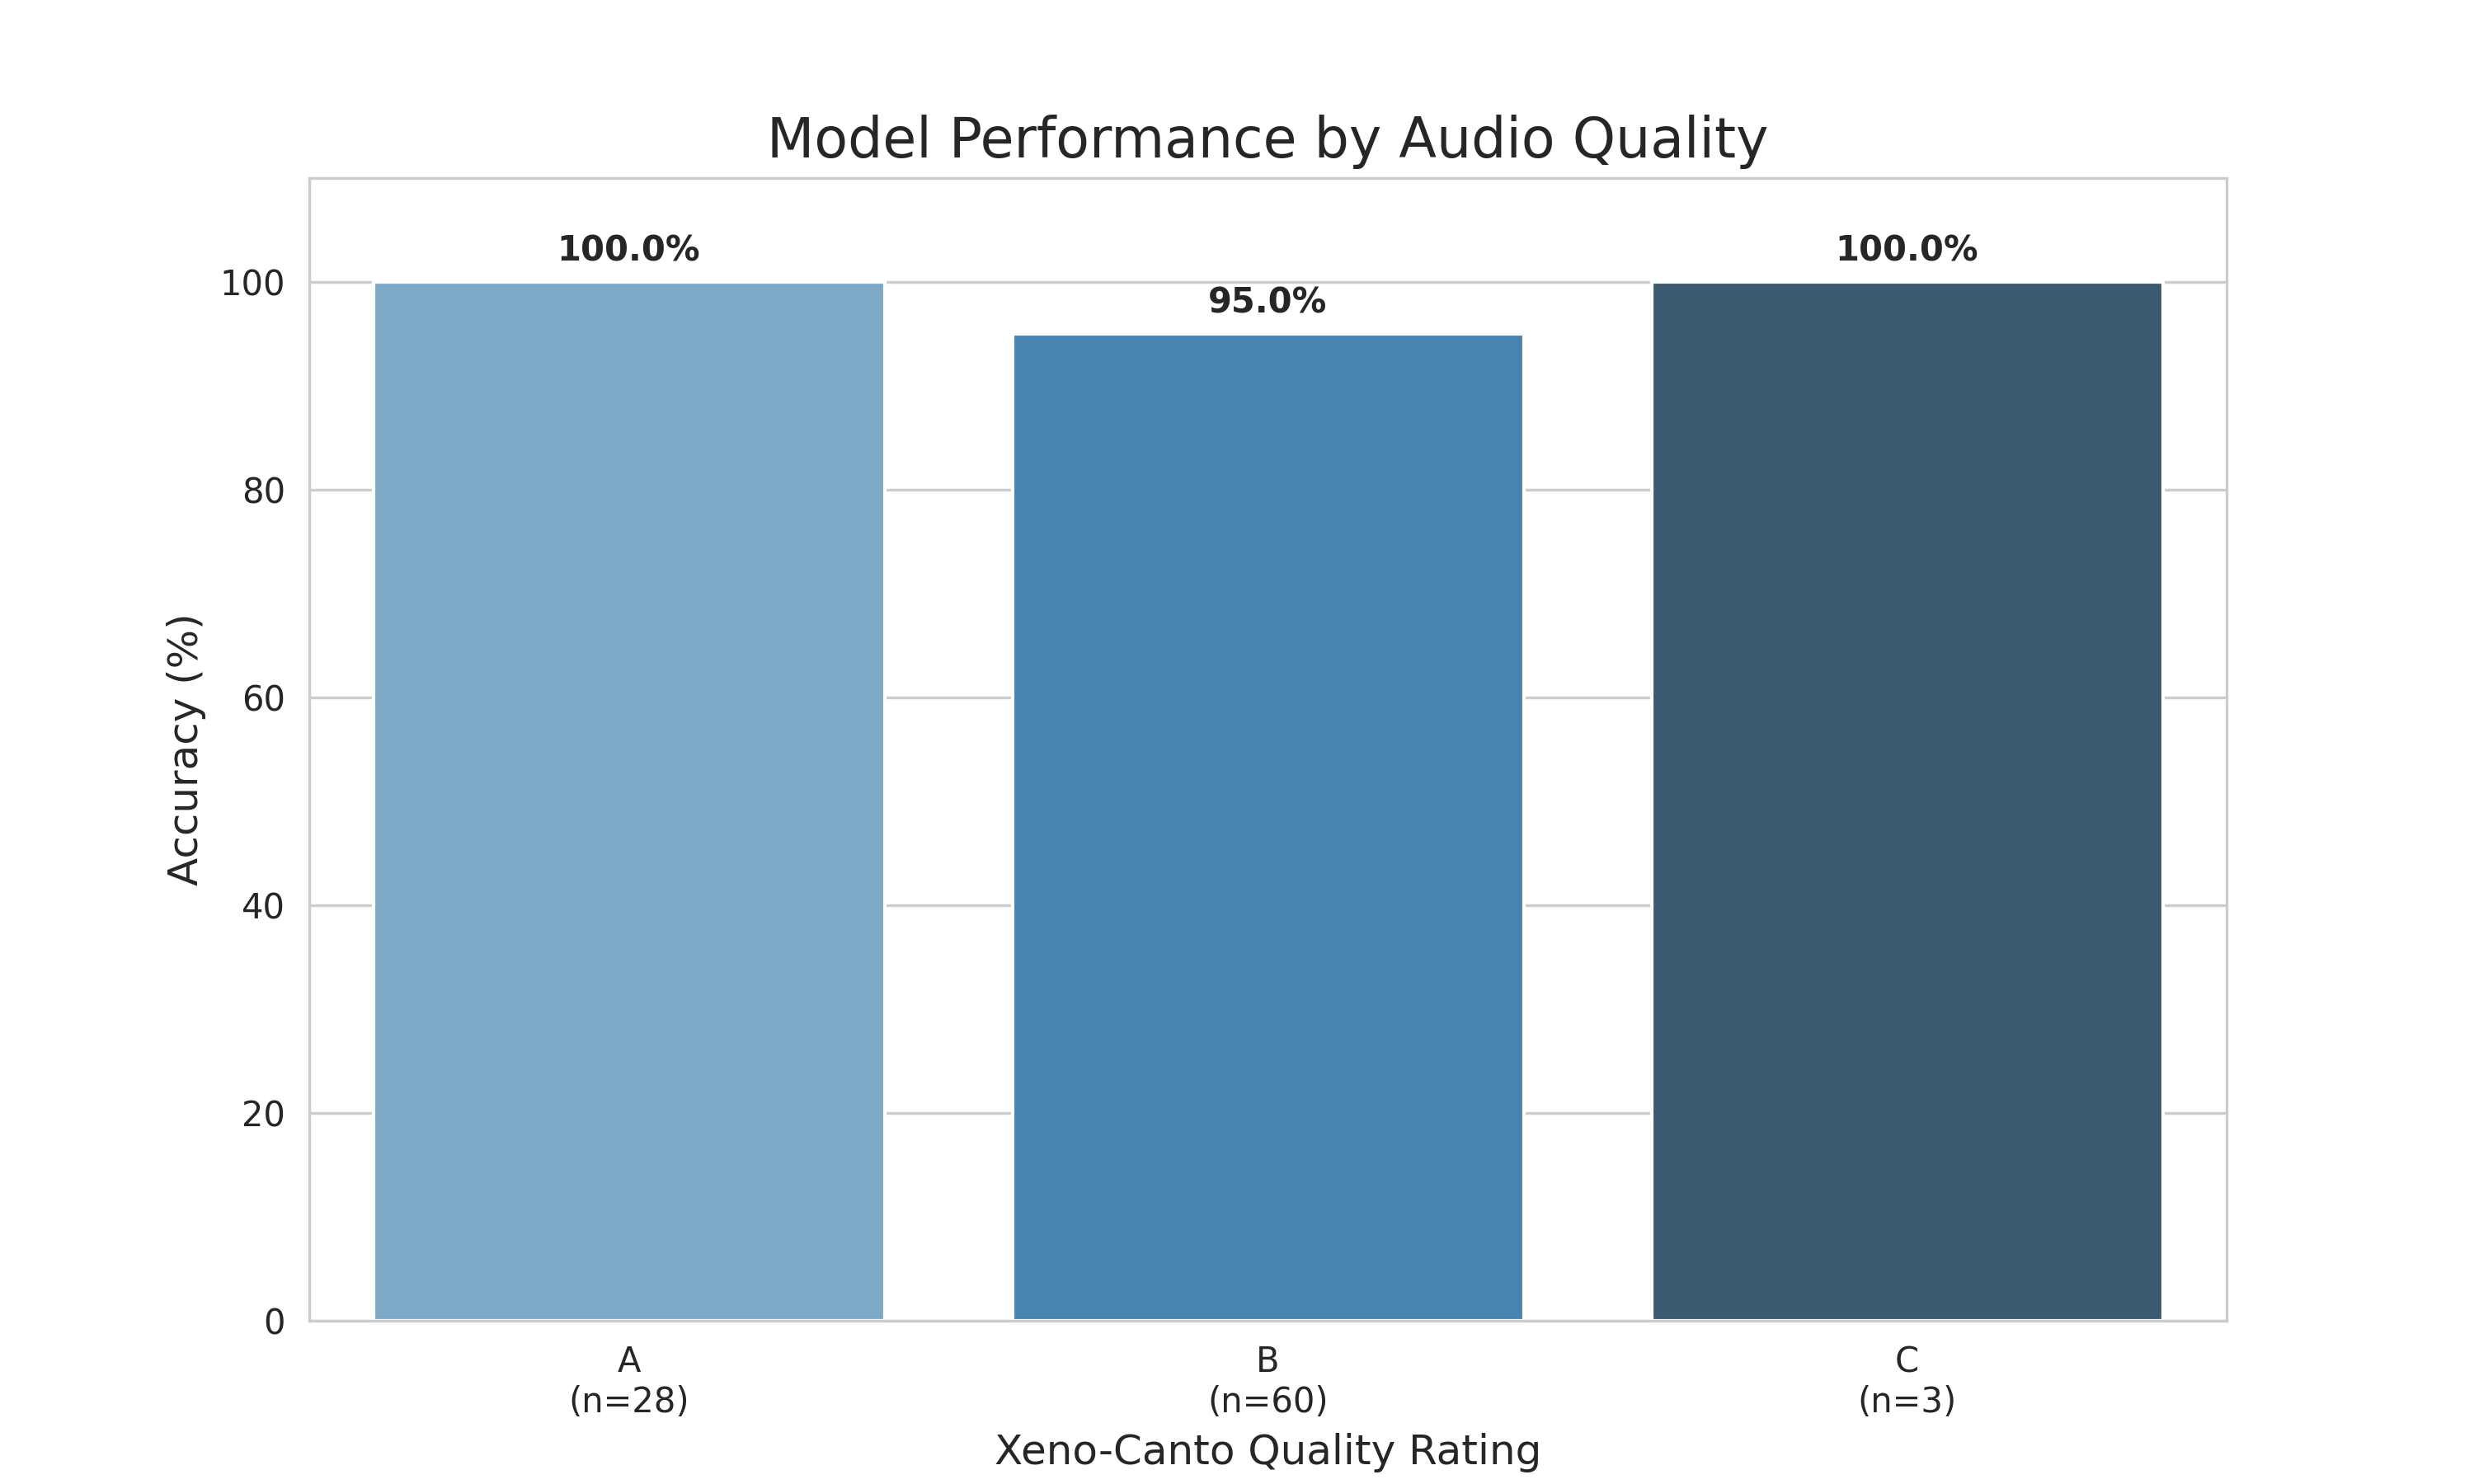
\includegraphics[width=0.7\textwidth]{Pictures/performance_by_quality.png}
    \caption{Performance nach Audioqualität. Selbst bei schlechten Aufnahmen (D/E) bleibt das Modell brauchbar.}
    \label{fig:quality}
\end{figure}

\subsection{Validierung durch externe Datenquellen (Cross-Testing)}
Ein häufiges Risiko beim Training neuronaler Netze ist der sogenannte \enquote{Dataset Bias} – das Modell lernt dabei nicht nur die Vogelstimmen, sondern versehentlich auch die spezifischen Eigenheiten der Aufnahmegeräte der Trainingsdatenbank. Um sicherzustellen, dass unser Modell generalisiert, haben wir Cross-Tests mit Audioquellen durchgeführt, die nicht Teil des Xeno-Canto-Trainingsdatensatzes waren.

Hierfür nutzten wir exemplarische Aufnahmen aus dem Google AudioSet sowie Referenzaufnahmen der Plattform \textit{kookoo.eu} (bekannt für hochwertige Singvogel-Aufnahmen). Das Modell konnte auch diese artfremden Aufnahmen mit hoher Zuverlässigkeit klassifizieren. Dies bestätigt, dass die KI tatsächlich die spektralen Muster der Vögel gelernt hat und nicht nur auf die akustische Signatur einer spezifischen Datenbank optimiert ist.


\subsection{Sliding Window Inference}
Im echten Einsatz bekommen wir keine vorgeschnittenen 5-Sekunden-Clips, sondern einen endlosen Audio-Stream. Wir nutzen daher einen \enquote{Sliding Window} Ansatz. Das Fenster schiebt sich über die Aufnahme und das Model gibt für jeden Moment eine Wahrscheinlichkeit aus.
In Abbildung \ref{fig:sliding} haben wir das visualisiert. Man sieht unten das Spektrogramm und oben drüber die Heatmap der KI Attention. Je heller (gelber/roter) die Farbe, desto sicherer ist sich die KI, dass dort ein Vogel singt. Man sieht schön, wie die KI genau bei den Gesangs-Events (hohe weiße Balken) ausschlägt.

\begin{figure}[H]
    \centering
    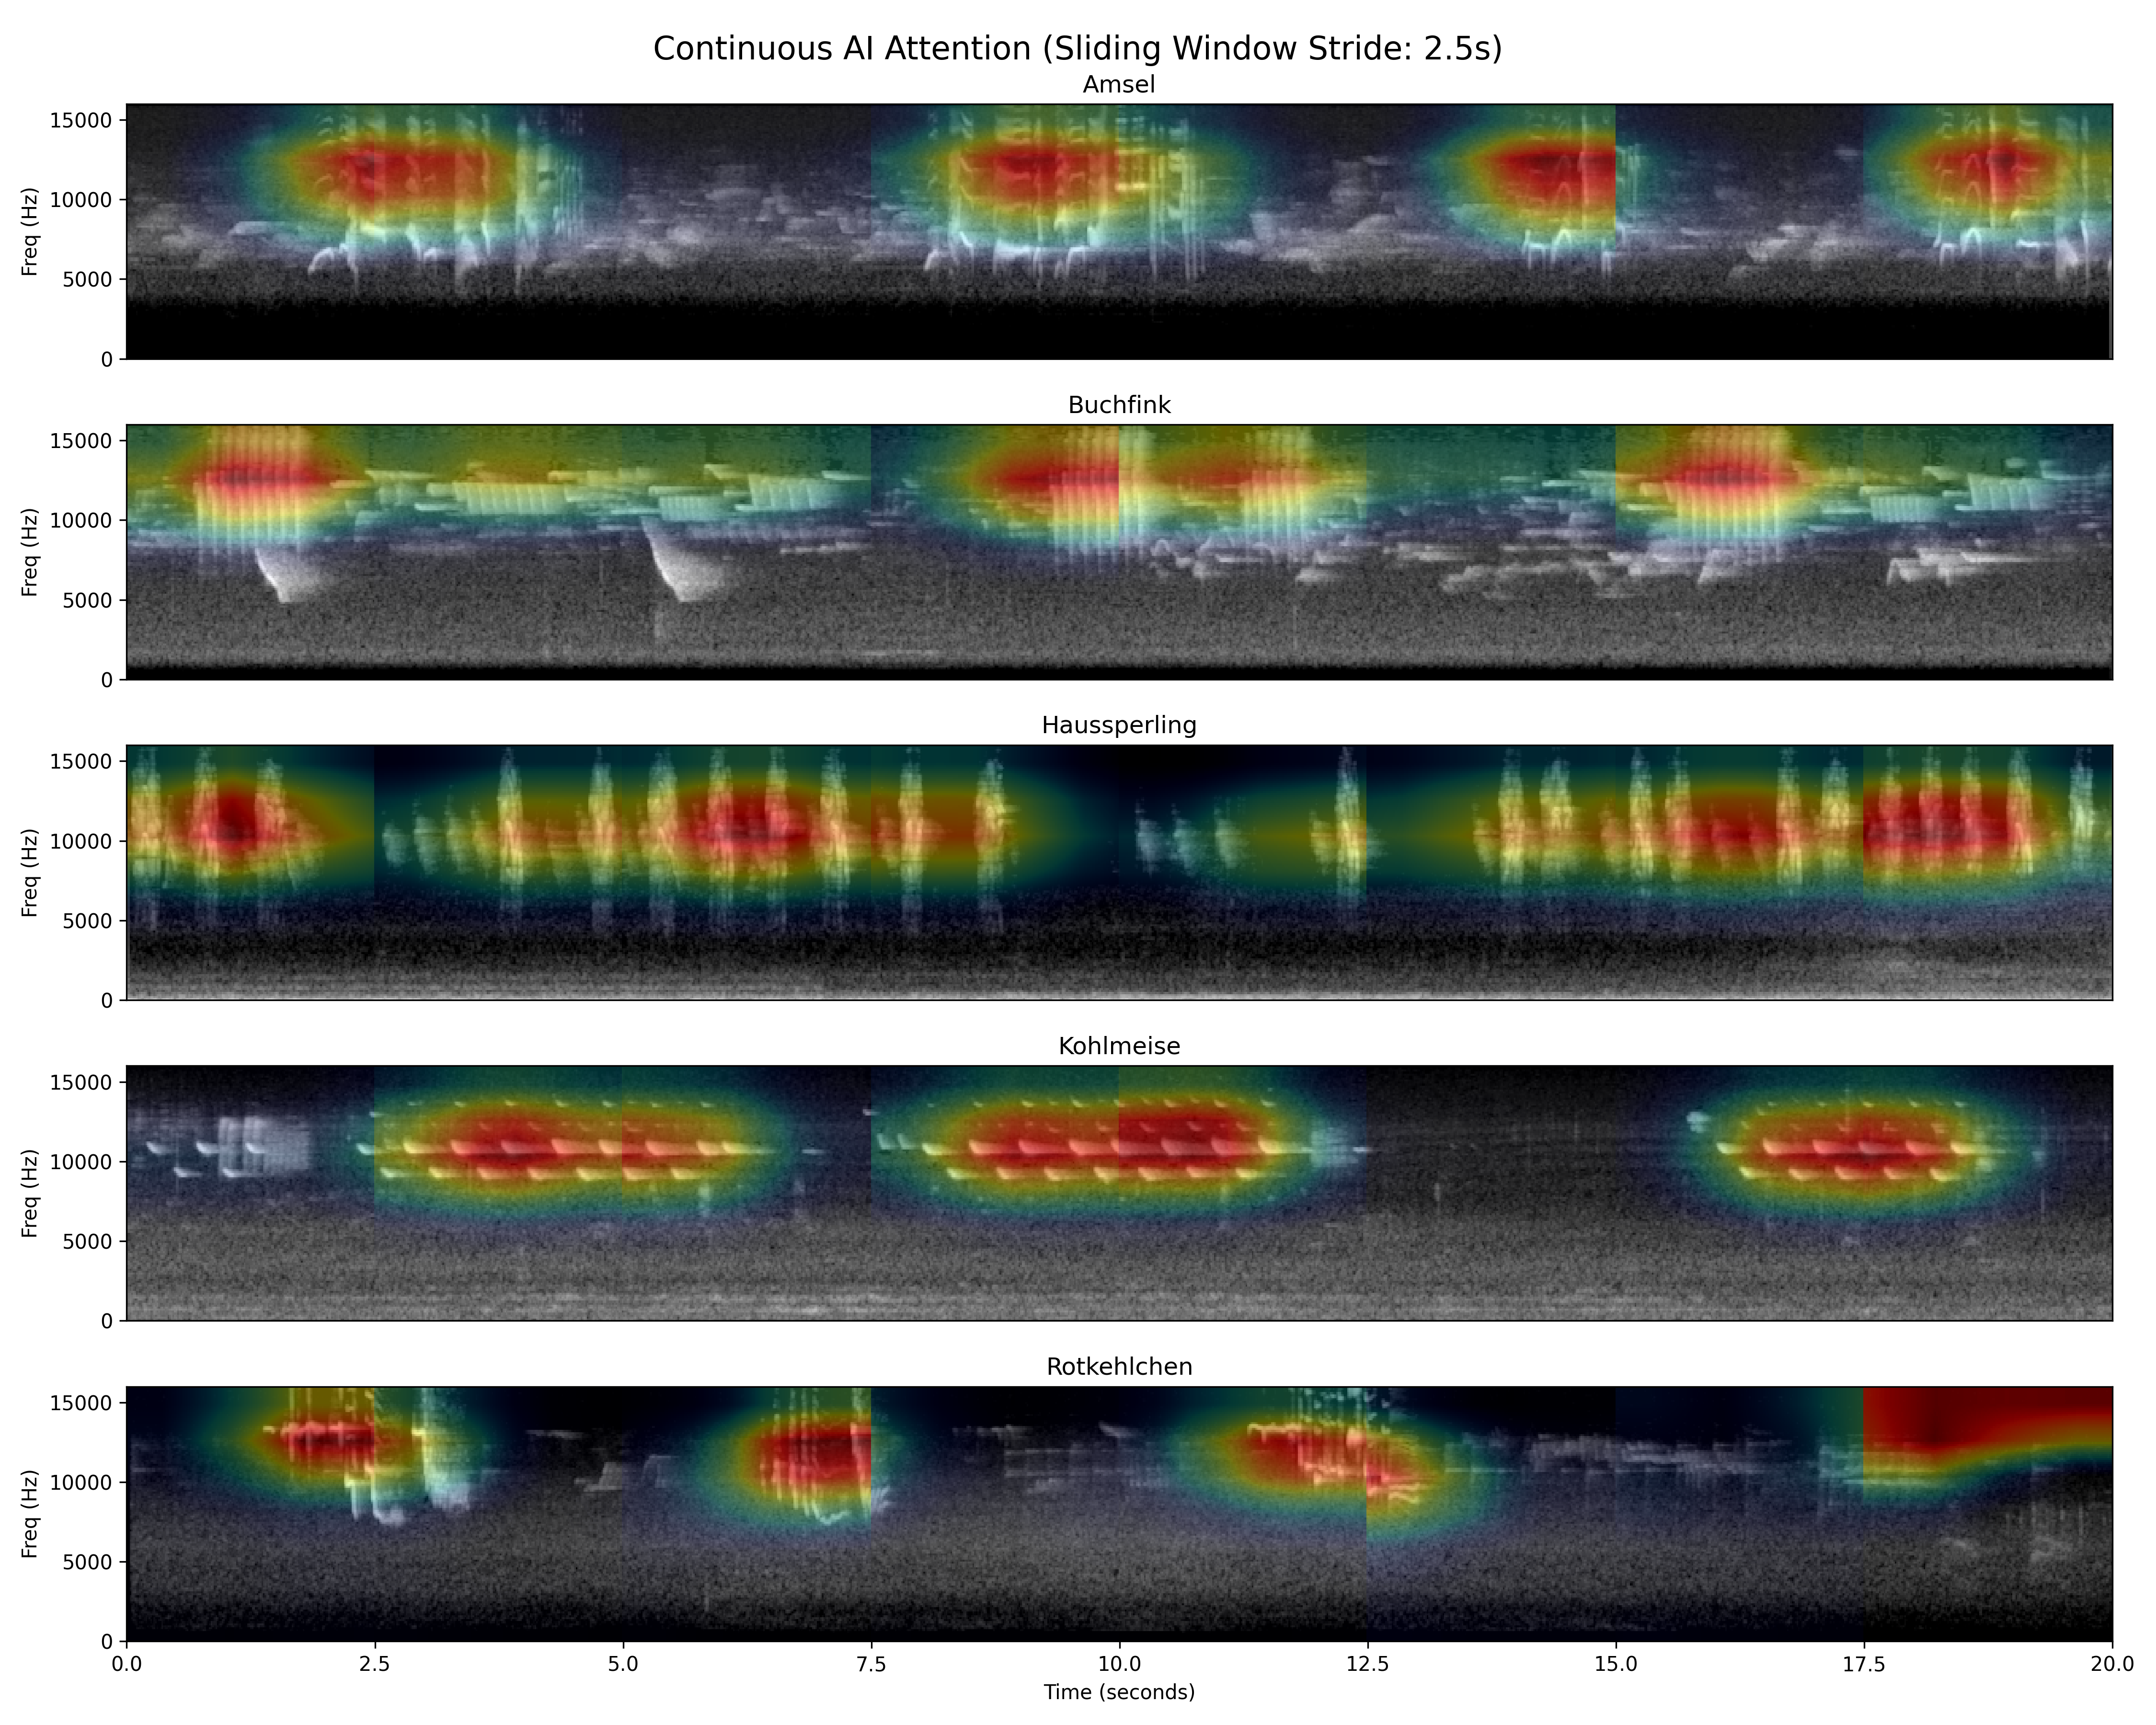
\includegraphics[width=1.0\textwidth]{Pictures/sliding_window_attention_2.5.png}
    \caption{Visualisierung der KI-Aufmerksamkeit. Die farbigen Bereiche markieren, wo das Modell relevante Merkmale im Audio-Stream gefunden hat.}
    \label{fig:sliding}
\end{figure}

\subsection{Zusatzexperimente: Rufe vs. Gesänge und Geschlecht}
Neben der Artenerkennung haben wir untersucht, ob das Modell auch den Typ der Lautäußerung (Gesang oder Ruf) unterscheiden kann. Die t-SNE Visualisierung der Embeddings (Abb. \ref{fig:tsne}) zeigt, dass das Modell diese Unterscheidung intern bereits lernt.
\begin{figure}[H]
    \centering
    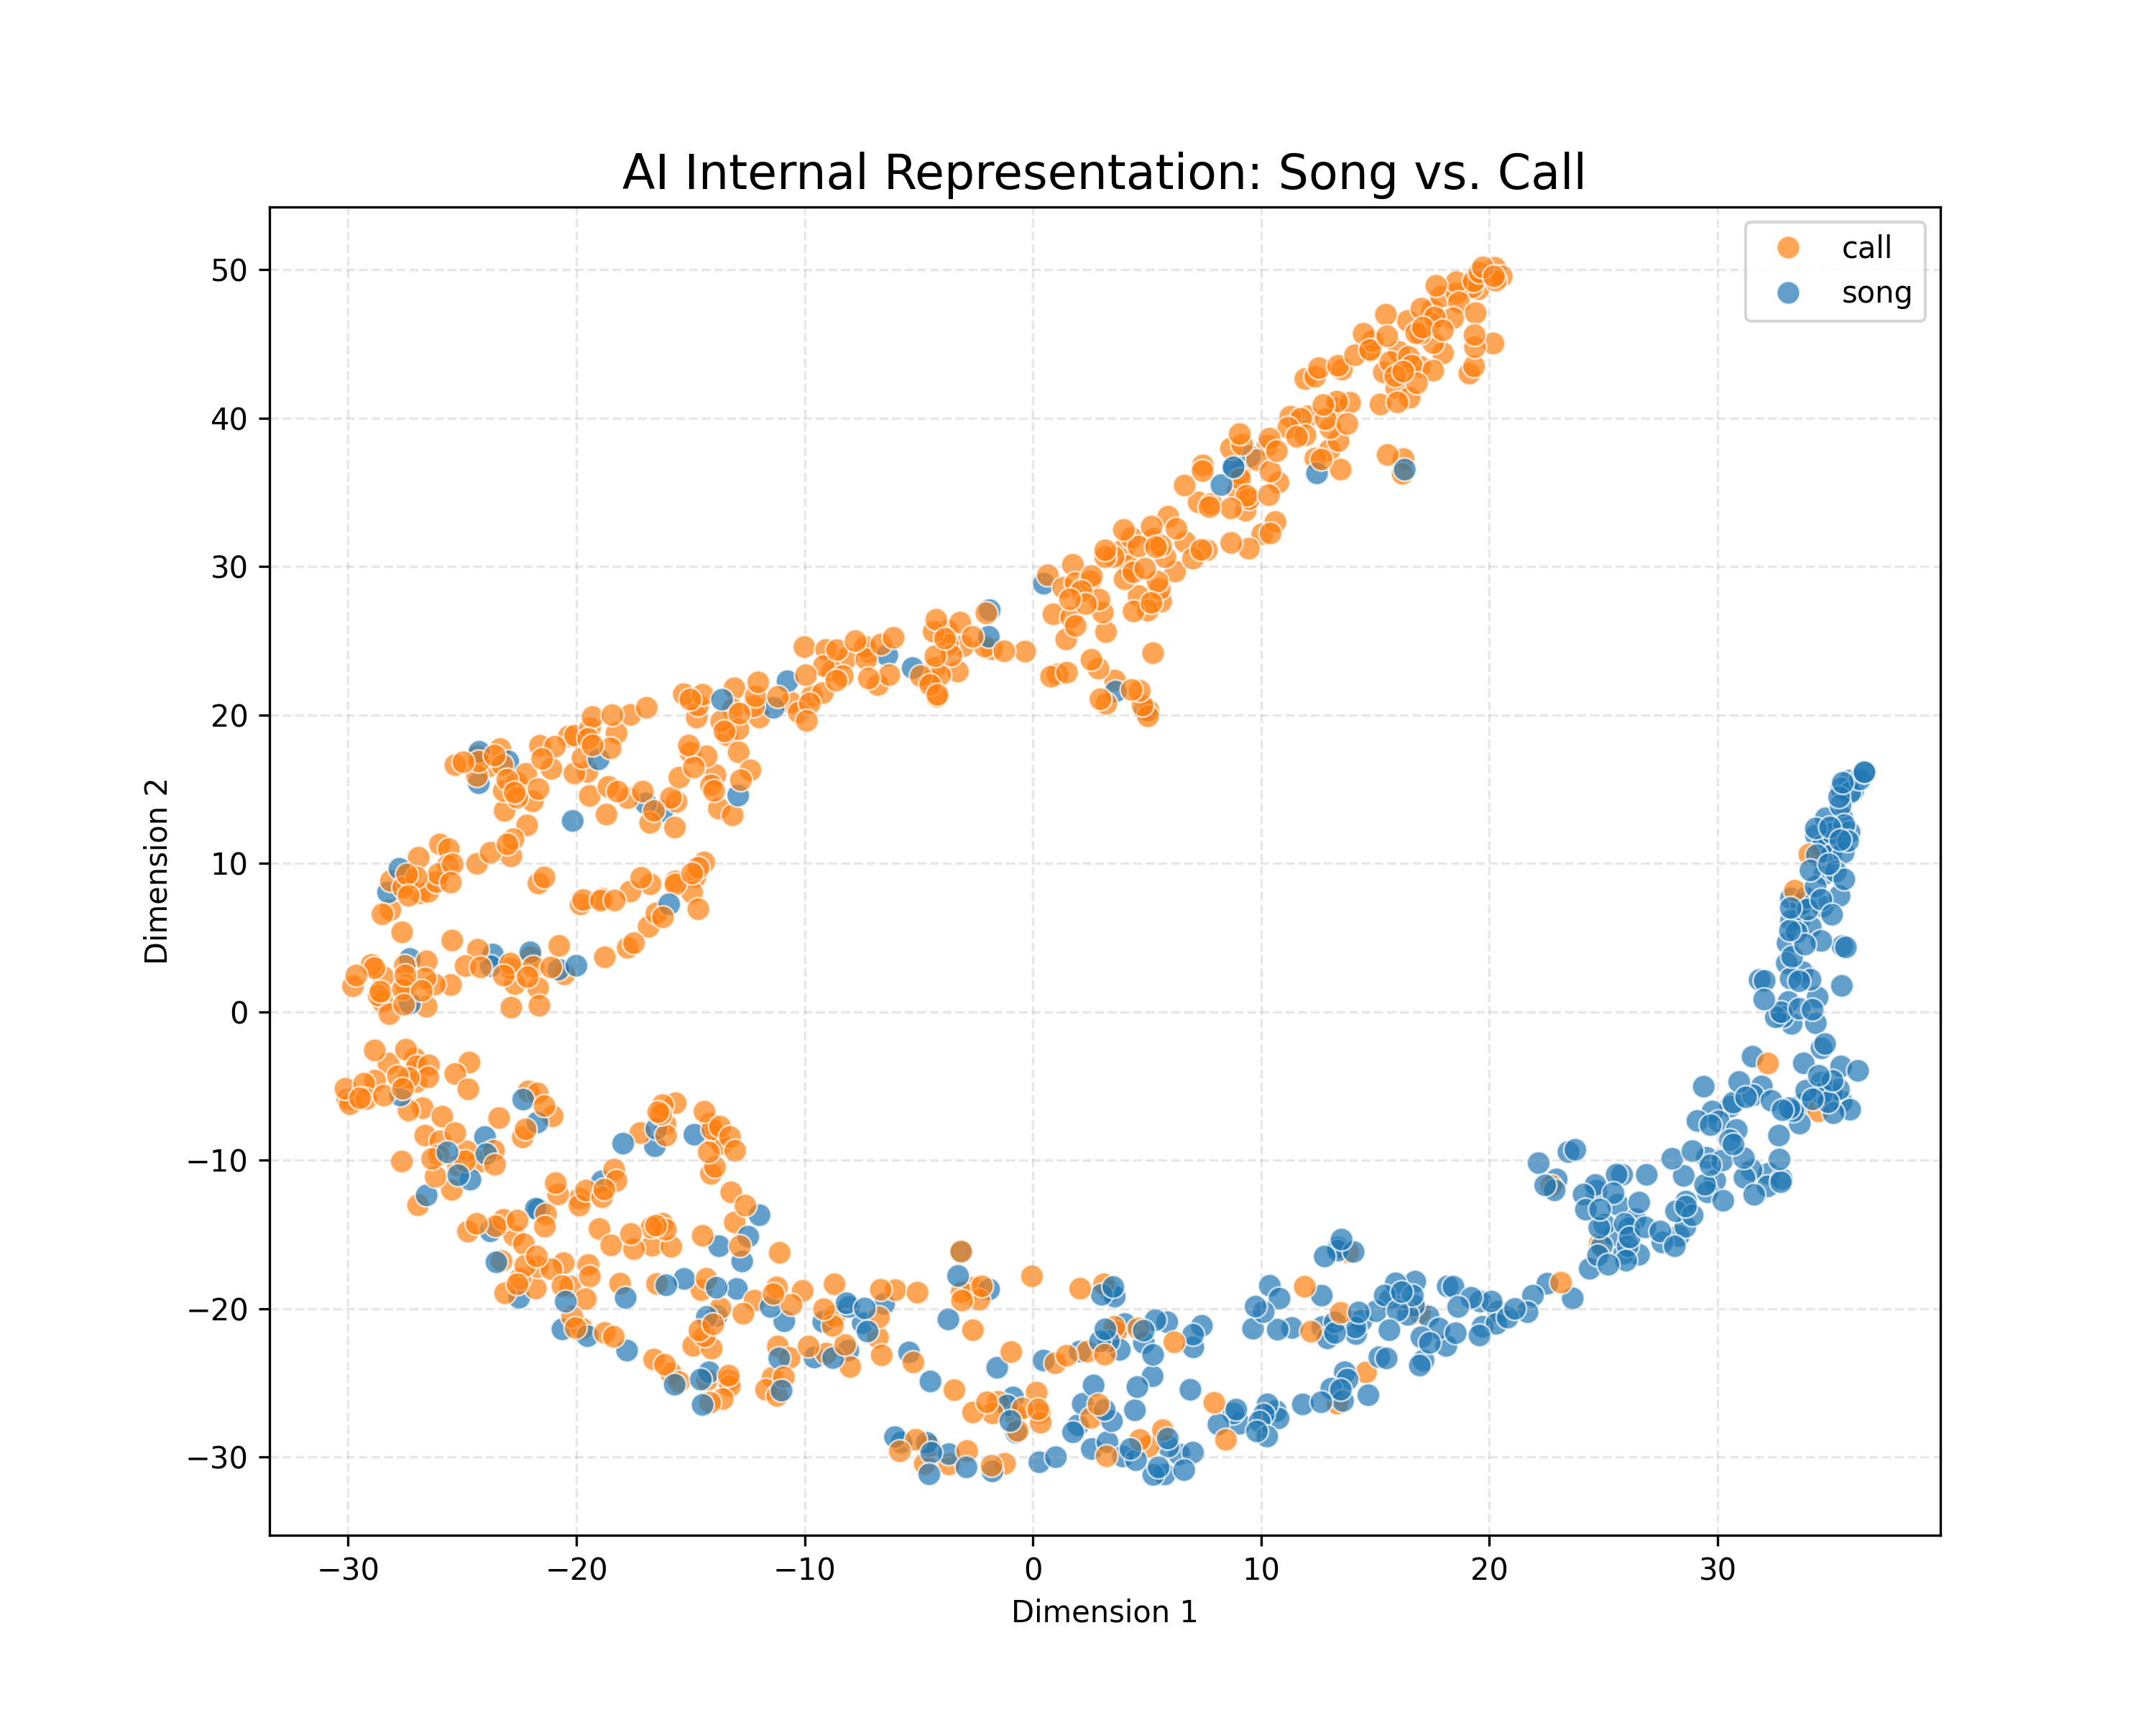
\includegraphics[width=0.8\textwidth]{Pictures/tsne_song_call.png}
    \caption{t-SNE Visualisierung der Modell-Embeddings. Rufe (Call) und Gesänge (Song) bilden teils eigene Cluster, auch ohne explizites Training darauf.}
    \label{fig:tsne}
\end{figure}

Zusätzlich haben wir getestet, ob ein auf Männchen-Daten gefiltertes Training bessere Ergebnisse liefert, da diese häufiger singen. Wie in Abbildung \ref{fig:gender} zu sehen, brachte die Einschränkung der Daten jedoch keinen statistisch signifikanten Vorteil gegenüber dem kompletten Datensatz.
\begin{figure}[H]
    \centering
    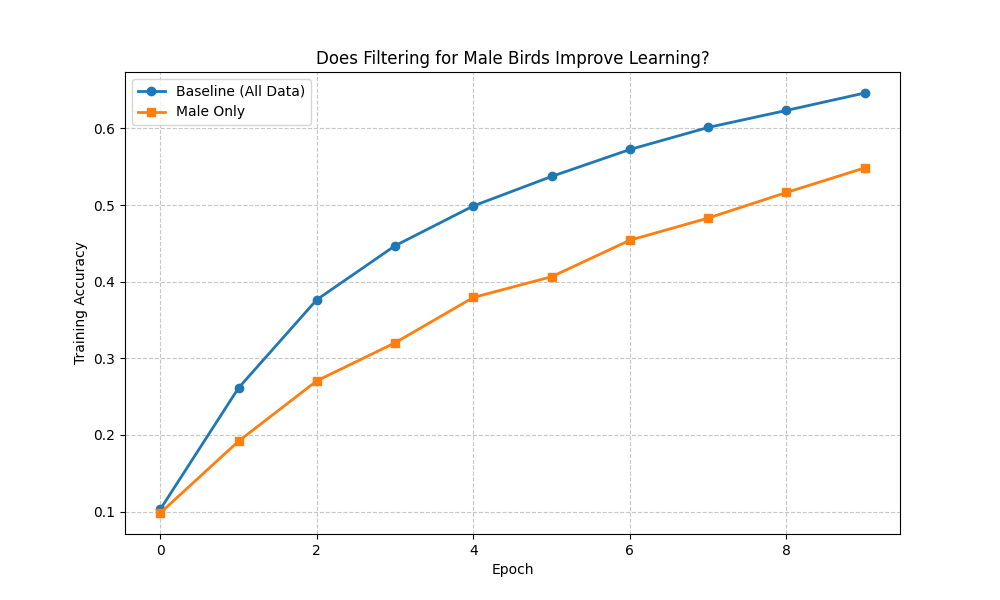
\includegraphics[width=0.8\textwidth]{Pictures/experiment_gender_result.png}
    \caption{Vergleich der Trainingsgenauigkeit: Das Filtern nach Geschlecht (Male Only) bringt keinen Vorteil gegenüber dem Nutzen aller Daten.}
    \label{fig:gender}
\end{figure}

\section{Hardware-Design}
Software ist nichts ohne Hardware. Mit \textit{Onshape} haben wir ein Gehäuse konstruiert, das alles zusammenhält.
Wichtig war uns, dass das Solarpanel direkt in den Deckel integriert ist, um den optimalen Winkel zur Sonne zu haben. Außerdem braucht das Mikrofon einen akustischen Trichter. Das Design ist modular aufgebaut, damit man Teile leicht austauschen kann, falls mal etwas kaputtgeht.

\begin{figure}[H]
    \centering
    \begin{subfigure}[b]{0.32\textwidth}
        \centering
        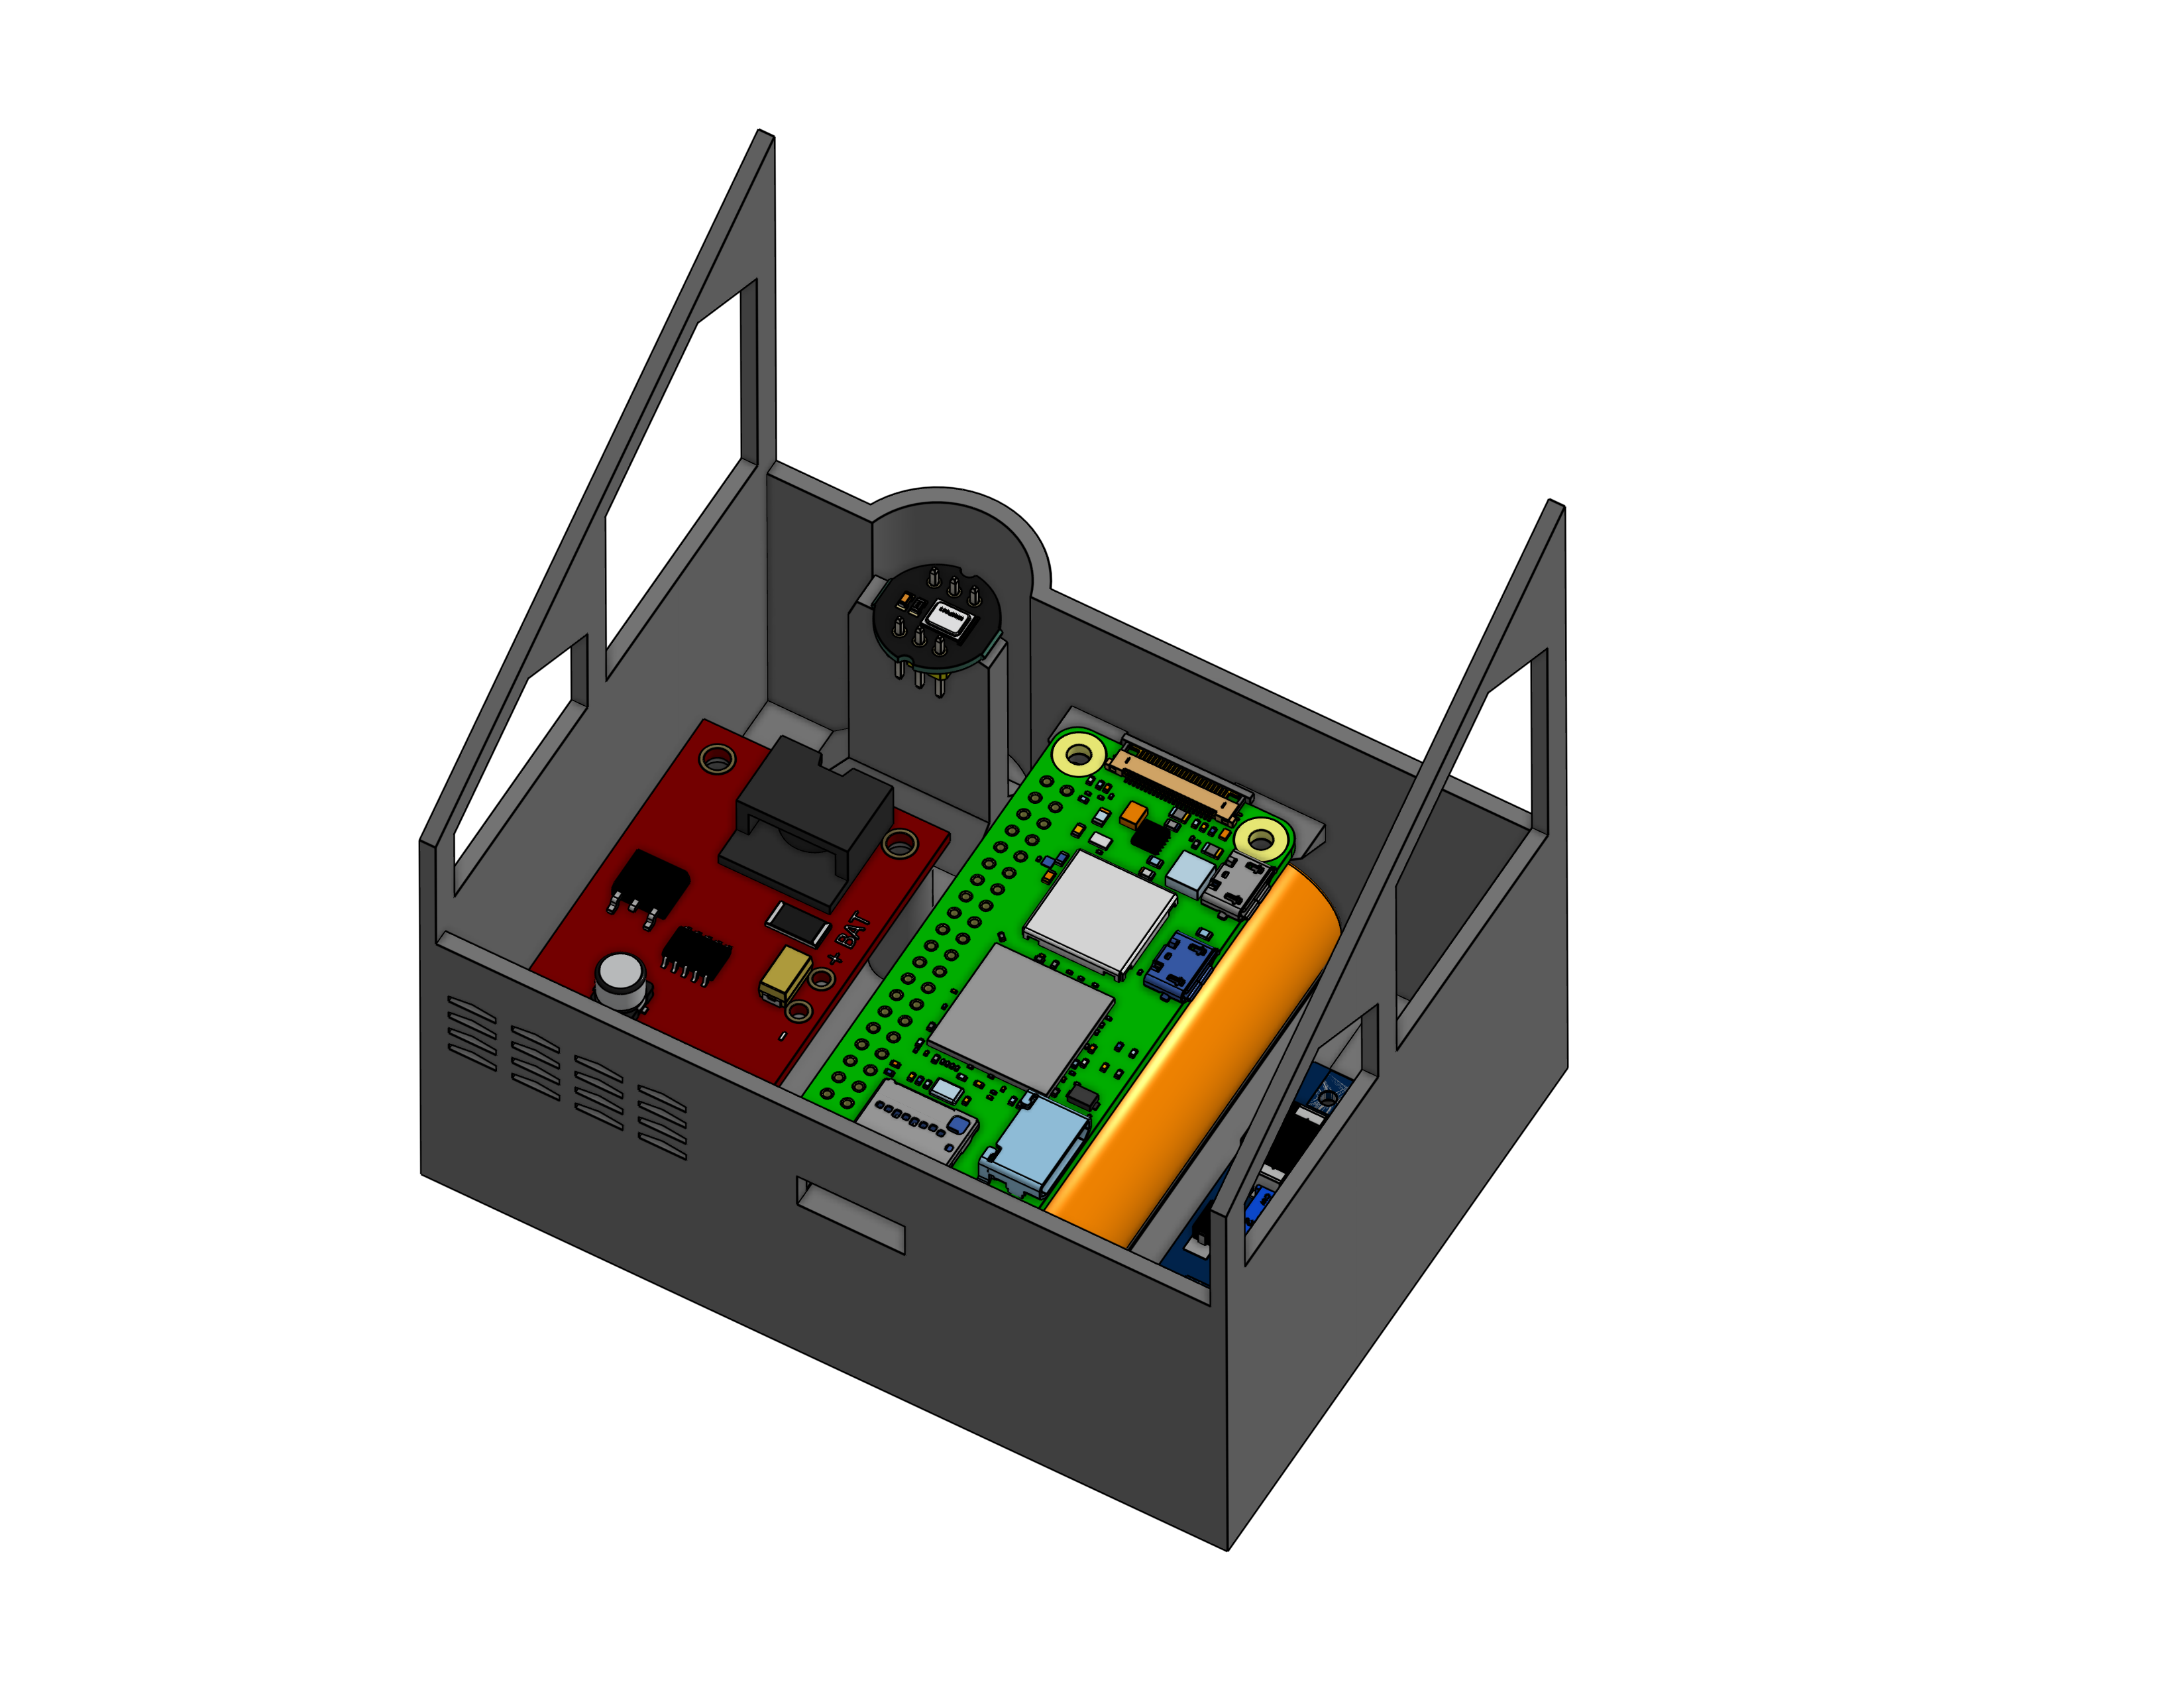
\includegraphics[width=\textwidth]{OnshapeImages/OnshapeModelView_CasingWithParts.png}
        \caption{Innenleben}
    \end{subfigure}
    \hfill
    \begin{subfigure}[b]{0.32\textwidth}
        \centering
        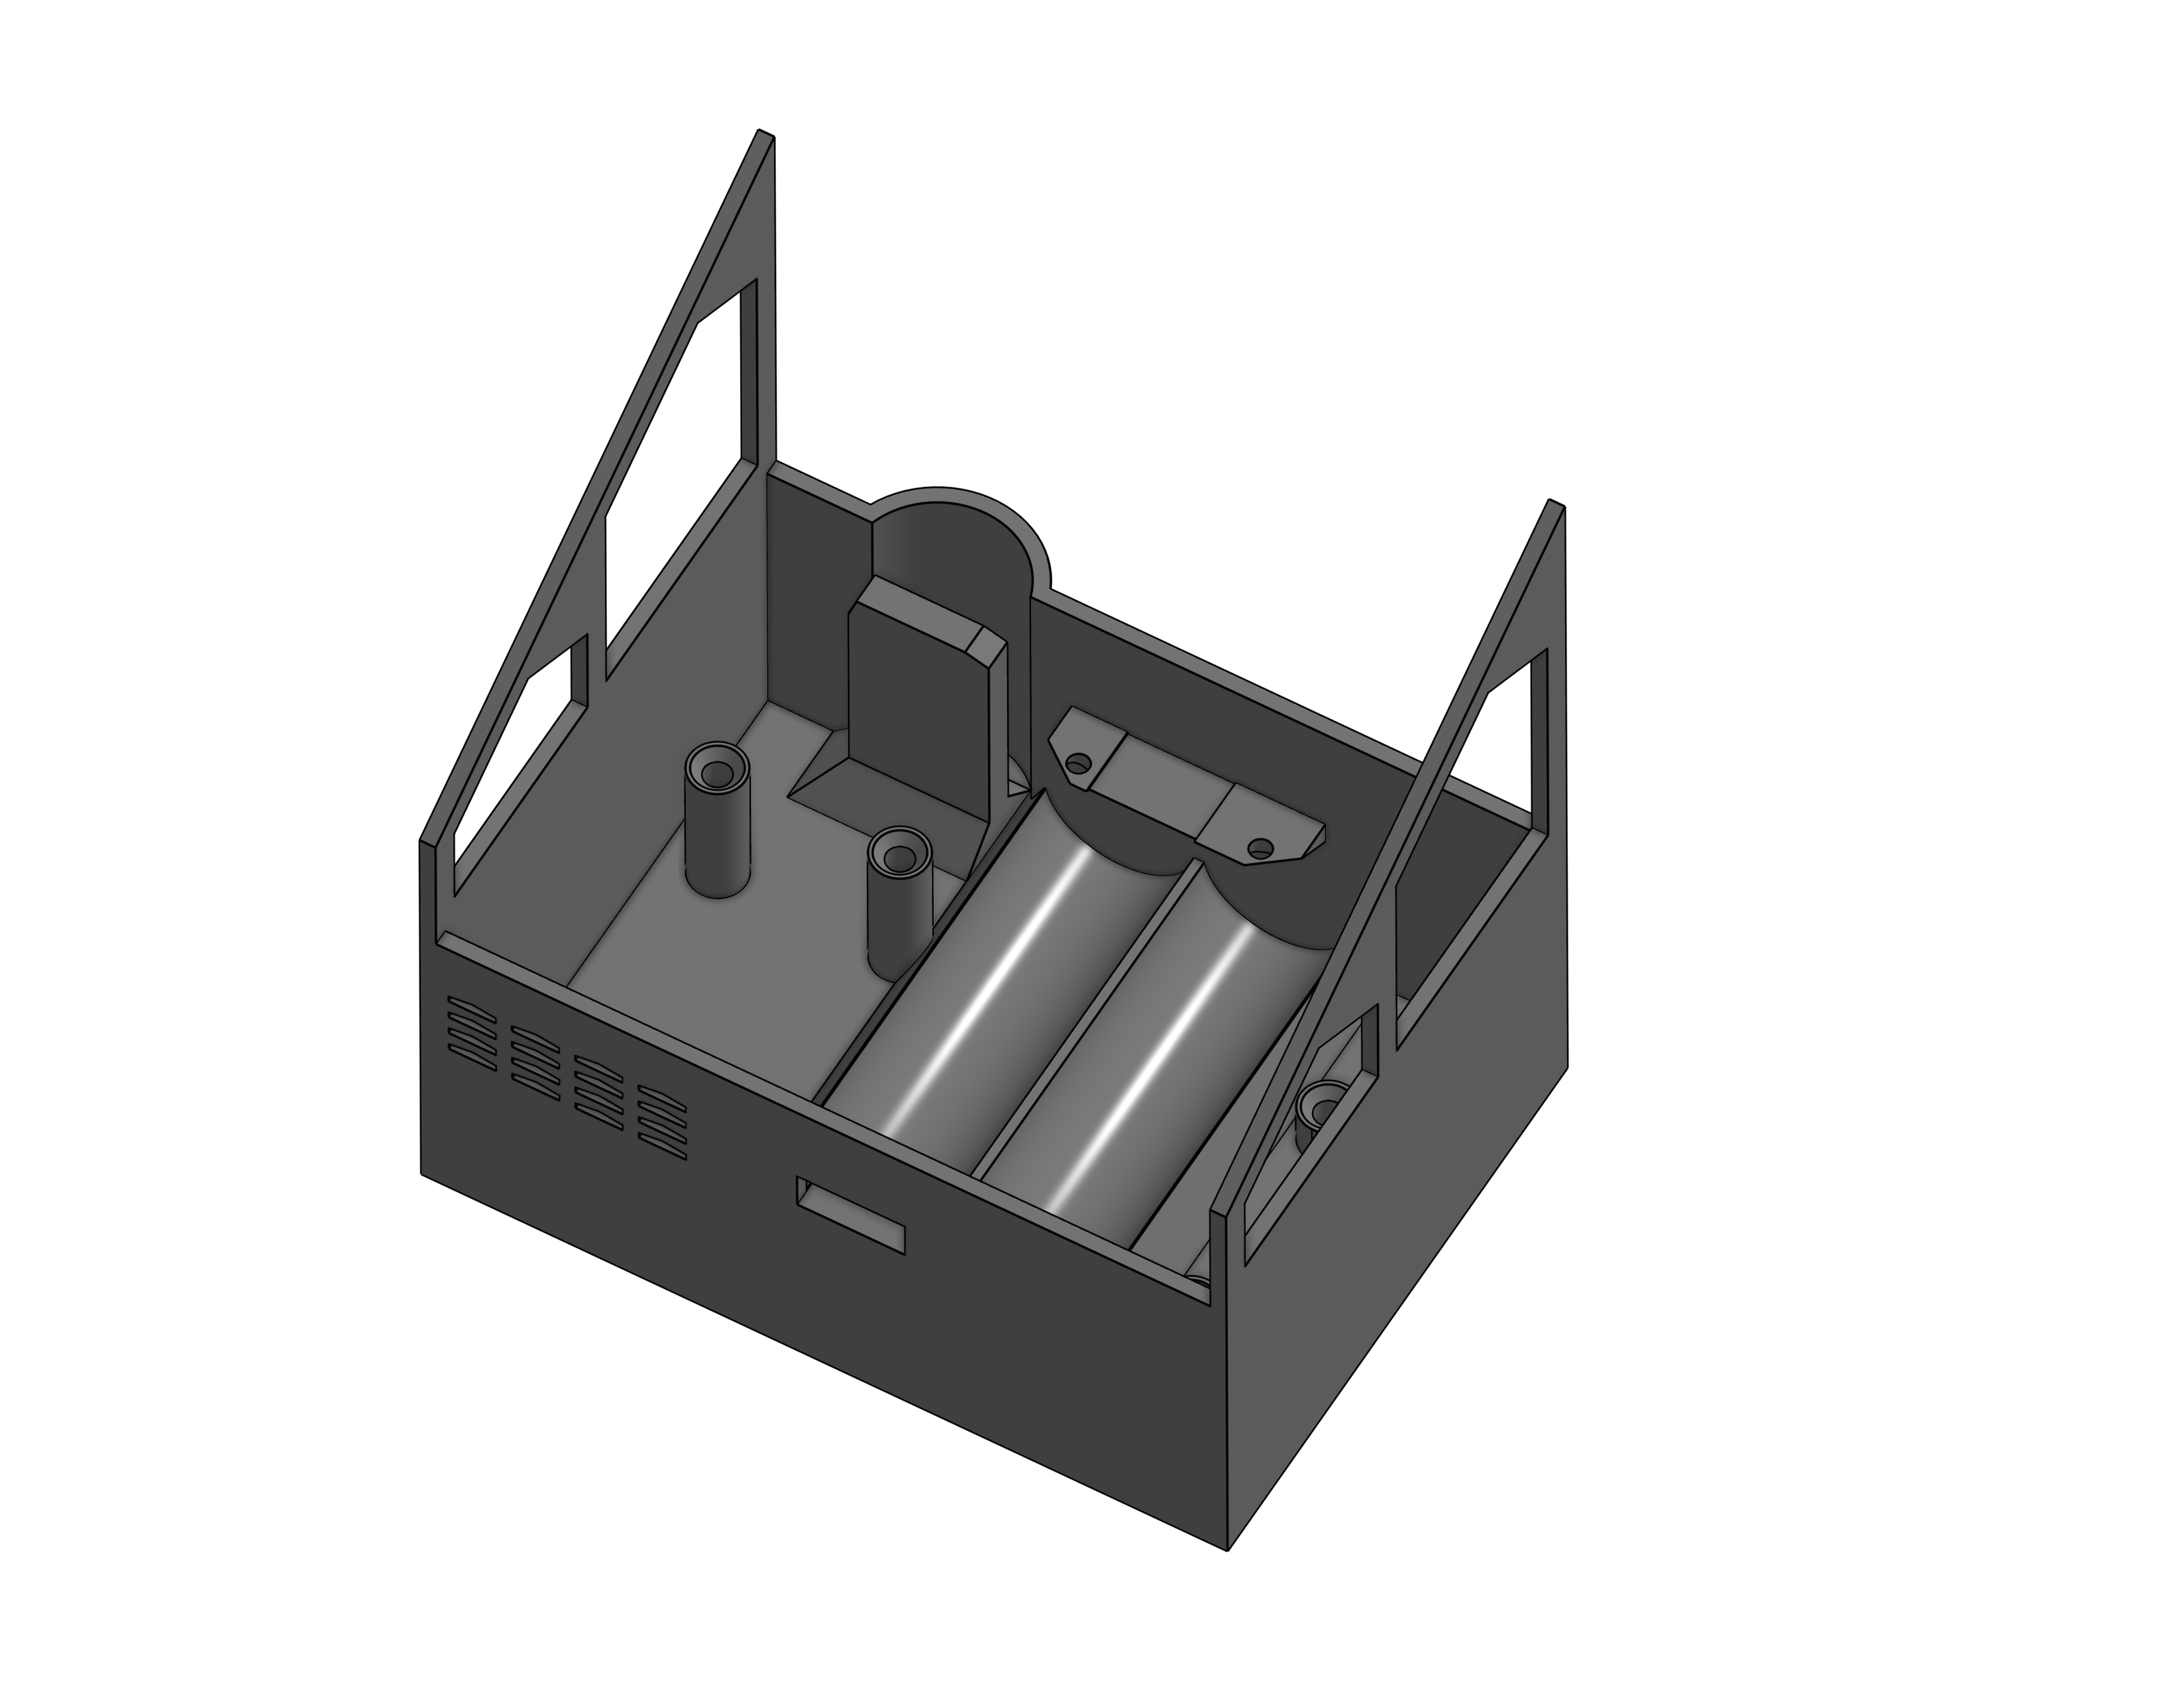
\includegraphics[width=\textwidth]{OnshapeImages/OnshapeModelView_OnlyCasing.png}
        \caption{Gehäuse-Struktur}
    \end{subfigure}
    \hfill
    \begin{subfigure}[b]{0.32\textwidth}
        \centering
        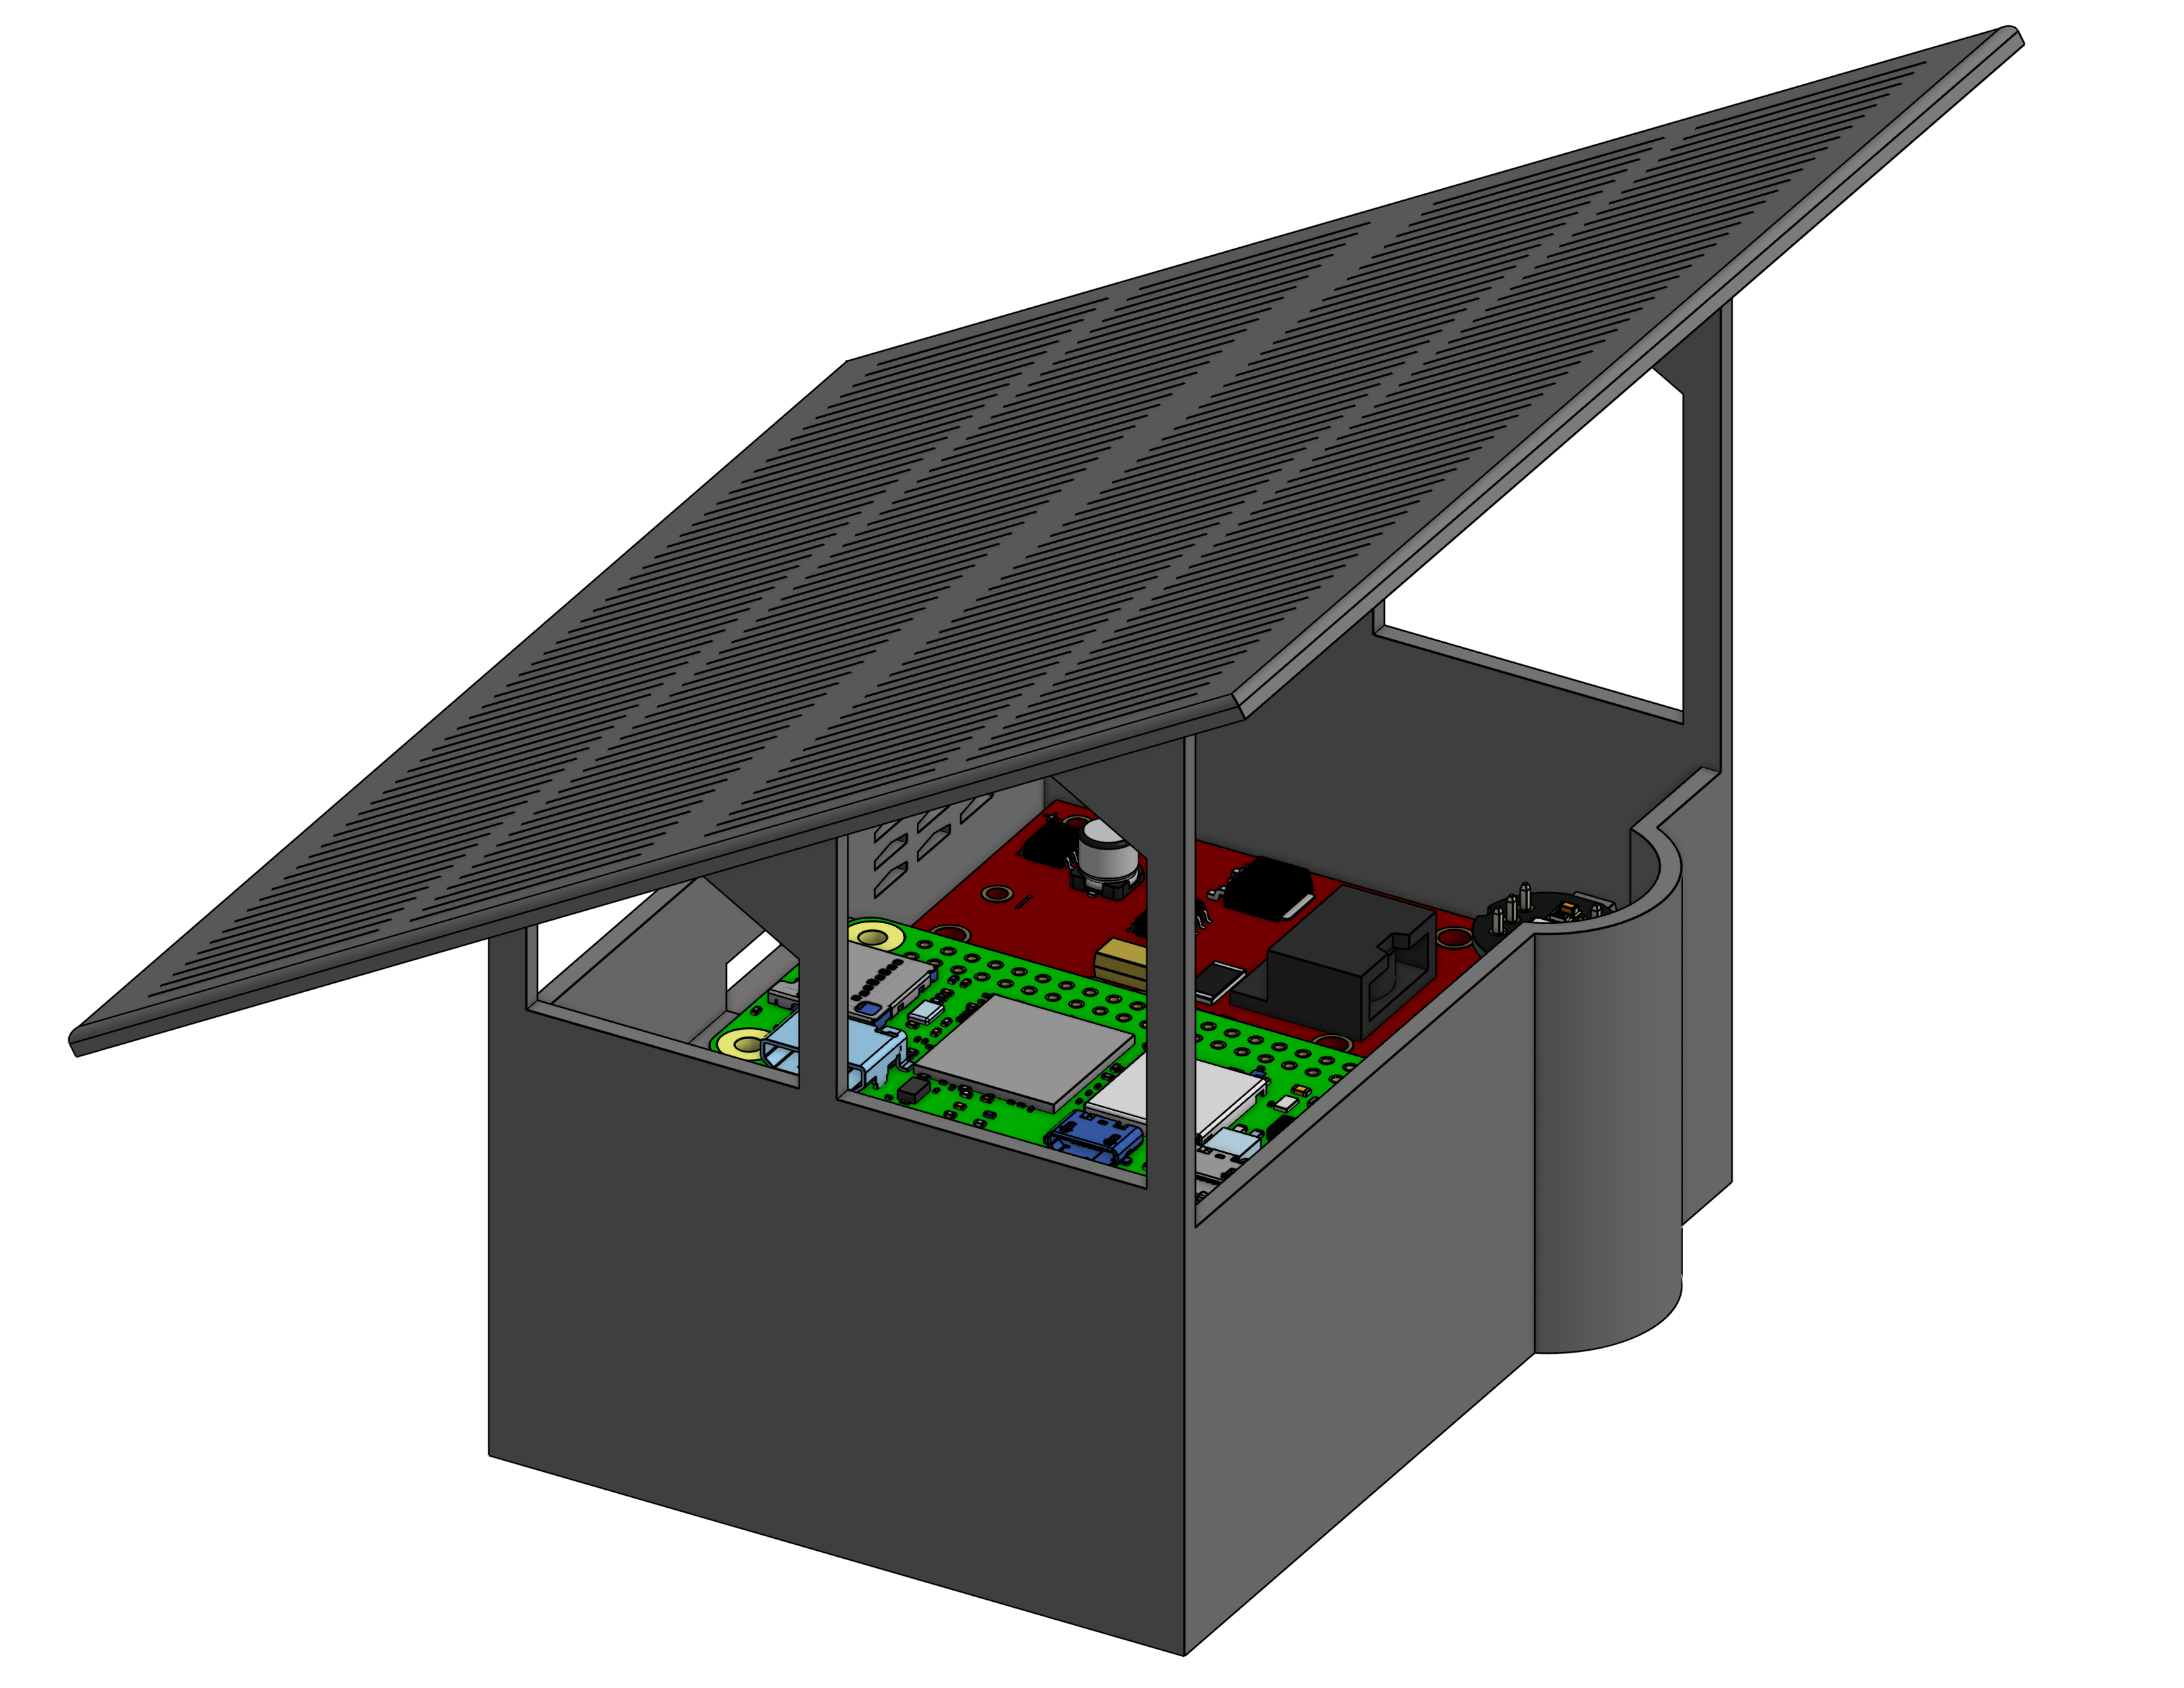
\includegraphics[width=\textwidth]{OnshapeImages/OnshapeModelView_SolarPanel.png}
        \caption{Solar-Integration}
    \end{subfigure}
    \caption{Unsere CAD-Konstruktion für den autonomen Feldeinsatz.}
    \label{fig:hardware}
\end{figure}

\section{Fazit und wie es weitergeht}
Wir haben gezeigt, dass es funktioniert. Die Software steht und liefert exzellente Werte. Besonders stolz sind wir darauf, dass wir mit Open-Source-Daten eine so hohe Genauigkeit erreichen konnten.
Was jetzt noch fehlt, ist der Härtetest im Wald. Wir müssen das Gehäuse drucken und schauen, ob der Raspberry Pi mit dem Solarstrom über den Winter kommt. Vielleicht müssen wir den Code noch effizienter machen oder auf Mikrocontroller wie den ESP32 umsteigen, um Strom zu sparen.
Außerdem wollen wir den \enquote{Sliding Window}-Algorithmus noch schneller machen, damit er direkt live auf dem Gerät laufen kann, ohne erst alles in die Cloud schicken zu müssen.

Ein entscheidender nächster Schritt für die wissenschaftliche Validierung ist der \enquote{Ground Truth}-Abgleich im Feld. Hierfür planen wir eine Kooperation mit der Experten-Community von \textit{BirdForum.net}. Ziel ist es, erfahrene Ornithologen oder Hobby-Beobachter zu gewinnen, die unsere Prototypen parallel zu ihren manuellen Beobachtungen einsetzen. Der Vergleich zwischen der KI-generierten Liste und den manuellen Notizen der Experten wird uns die verlässlichsten Daten über die Performance unter realen Bedingungen (IRL-Tests) liefern.

% --- Literaturverzeichnis ---
\newpage
\renewcommand\refname{Quellen- und Literaturverzeichnis}
\begin{thebibliography}{9}

\bibitem{kahl2021}
Kahl, S., et al. (2021).
\textit{BirdNET: A deep learning solution for avian diversity monitoring.}
Ecological Informatics.

\bibitem{tan2019}
Tan, M., \& Le, Q. V. (2019).
\textit{EfficientNet: Rethinking Model Scaling for Convolutional Neural Networks.}
arXiv preprint arXiv:1905.11946.

\bibitem{specaugment}
Park, D. S., et al. (2019).
\textit{SpecAugment: A Simple Data Augmentation Method for Automatic Speech Recognition.}
Proc. Interspeech 2019.

\bibitem{xenocanto}
Xeno-Canto Foundation.
\textit{Xeno-canto: Sharing bird sounds from around the world.}
\url{https://www.xeno-canto.org/}

\end{thebibliography}

% --- Unterstützungsleistungen ---
\newpage
\section*{Unterstützungsleistungen}
Daten und Programme  der Open-Source-Community haben die Umsetzung unseres Projekts erleichtert. Insbesondere die Audiodaten von Xeno-Canto waren essenziell. Für die Programmierung haben wir Bibliotheken wie PyTorch, Librosa und Audiomentations genutzt. Ohne diese Tools wäre das Projekt in der Zeit gar nicht machbar gewesen. Ein Dank geht auch an unsere Informatik-Lehrer für das Feedback zwischendurch.

Ein besonderer Dank geht an David May für die Gestaltung des Titelbildes sowie an unsere JuFo-Lehrer für die Betreuung unseres Projekts.

\end{document}
